%%%%%%%%%%%%%%%%%%%%%%%%%%%%%%%%%%%%%%%%%%%%%%%%%%%%%%%%%%%%%%
%
% Welcome to Overleaf --- just edit your LaTeX on the left,
% and we'll compile it for you on the right. If you open the
% 'Share' menu, you can invite other users to edit at the same
% time. See www.overleaf.com/learn for more info. Enjoy!
%
%%%%%%%%%%%%%%%%%%%%%%%%%%%%%%%%%%%%%%%%%%%%%%%%%%%%%%%%%%%%%%%
% \documentclass[]{interact}

% \usepackage{epstopdf}% To incorporate .eps illustrations using PDFLaTeX, etc.
% \usepackage[caption=false]{subfig}% Support for small, `sub' figures and tables
% %\usepackage[nolists,tablesfirst]{endfloat}% To `separate' figures and tables from text if required
% %\usepackage[doublespacing]{setspace}% To produce a `double spaced' document if required
% %%-----------------------------
% \usepackage[numbers,sort&compress]{natbib}% Citation support using natbib.sty
% \bibpunct[, ]{[}{]}{,}{n}{,}{,}% Citation support using natbib.sty
% \renewcommand\bibfont{\fontsize{10}{12}\selectfont}% Bibliography support using natbib.sty
% \makeatletter% @ becoeez,ez ZZ e ¢33333 fffff f  ff fxxffff fx xcfxx f fmes a letter
% \def\NAT@def@citea{\def\@citea{\NAT@separator}}% Suppress spaces between citations using natbib.sty
% \makeatother% @ becomes a symbol again

% \theoremstyle{plain}% Theorem-like structures provided by amsthm.sty
% \newtheorem{theorem}{Theorem}[section]
% \newtheorem{lemma}[theorem]{Lemma}
% \newtheorem{corollary}[theorem]{Corollary}
% \newtheorem{proposition}[theorem]{Proposition}

% \theoremstyle{definition}
% \newtheorem{definition}[theorem]{Definition}
% \newtheorem{example}[theorem]{Example}

% \theoremstyle{remark}
% \newtheorem{remark}{Remark}
% \newtheorem{notation}{Notation}

% \usepackage[T1]{fontenc}
% \usepackage[utf8]{inputenc}
% \usepackage{lmodern}

% \usepackage[english]{babel}
% \usepackage{csquotes}

% \usepackage[notes,backend=biber]{biblatex-chicago}
% \bibliography{interactnlmsample}



\documentclass[]{article}
\usepackage[toc]{glossaries}
% \usepackage[utf8]{inputenc}
%  \usepackage[acronym]{glossaries}

\makeglossaries

\newglossaryentry{Artificial Intelligence}
{
    name=Artificial Intelligence,
    description={Artificial intelligence (AI) is the intelligence of machines or software, as opposed to the intelligence of humans or other animals. It is a field of study in computer science that develops and studies intelligent machines. Such machines may be called AIs.}
}
\newglossaryentry{Autonomous Forces}
{
    name=Autonomous Forces,
    description={Autonomous forces are military systems that can operate without human intervention. They are often used in unmanned vehicles, drones, and other military equipment. The Department of Defense has hypothesized that future demand for uncrewed systems will strain the capacity of the defense industrial base.}
}
\newglossaryentry{combat modeling}
{
    name=combat modeling,
     description={Combat Modeling focuses on the challenges in human, social, cultural, and behavioral modeling such as the core processes of move, shoot, look, and communicate within a synthetic environment and also equips readers with the knowledge to fully understand the related concepts and limitations.}
}
\newglossaryentry{deep learning}
{
    name=deep learning,
     description={Deep learning is a type of machine learning that uses artificial neural networks to learn from data. Artificial neural networks are inspired by the human brain, and they can be used to solve a wide variety of problems, including image recognition, natural language processing, and speech recognition.}
}

\newglossaryentry{latex}
{
    name=latex,
    description={Is a markup language specially suited 
    for scientific documents}
}

\newglossaryentry{maths}
{
    name=mathematics,
    description={Mathematics is what mathematicians do}
}
\newglossaryentry{Military Strategy}
{
    name=Military Strategy,
    description={Military Strategy is the planning and execution of the contest between groups of armed adversaries. It involves using all the military, economic, political, and other resources of a country to achieve the objectives of war. Military strategy is often divided into four components: ends (objectives), ways (courses of action), means (resources), and risk.
    Military strategy has a long history, dating back to ancient times. Some of the most influential thinkers on military strategy include Sun Tzu, Machiavelli, Clausewitz, Jomini, Liddell Hart, and others. Military strategy is influenced by the nature of warfare, the characteristics of the adversaries, the goals of the policy, and the constraints of the environment. Military strategy is not static, but dynamic and adaptive to changing circumstances}
}

\newglossaryentry{formula}
{
        name=formula,
        description={A mathematical expression}
}
\newglossaryentry{rlNumericSpace}
{
        name=rlNumericSpace,
        description={A Continuous observations or actions space in Reinforcement Learning}
}
\newglossaryentry{rlFiniteSetSpace}
{
        name=rlFiniteSetSpace,
        description={A discrete observations or actions space in Reinforcement Learning}
}
\newglossaryentry{Withdrawal}
{
        name=Withdrawal,
        description={A tactical withdrawal or retreating defensive action is a type of military operation, generally meaning that retreating forces draw back while maintaining contact with the enemy. }
}
\newglossaryentry{Breakthrough}
{
        name=Breakthrough,
        description={A breakthrough occurs when an offensive force has broken or penetrated an opponent's defensive line, and rapidly exploits the gap.}
}
\newglossaryentry{Delaying}
{
        name=Delaying,
        description={a defensive military action in which advance of an enemy is delayed by fighting as long as possible without the defensive force becoming involved in decisive battle that would imperil its withdrawal}
}
\newglossaryentry{Stalemate}
{
        name=Stalemate,
        description={Stalemate is a situation in chess where the player whose turn it is to move is not in check and has no legal move.}
}
\newglossaryentry{Hasty Defense}
{
        name=Hasty Defense,
        description={Hasty Defense - this is a defense you assume when you are in immediate contact with the enemy. }
}
\newglossaryentry{Deliberate Defense}
{
        name=Deliberate Defense,
        description={a defense organized before contact is made with the enemy and while time for organization is available; usually includes a fortified zone (with pillboxes) and communication systems}
}
\newglossaryentry{Prepared Defense}
{
        name=Prepared Defense,
        description={ preparedness requires considerable and consistent conceptual clarity, 
        facile ground 
        (defPrep=70\%)}
}
\newglossaryentry{Fortified Defense}
{
        name=Fortified Defense,
        description={A fortification (also called a fort, fortress, or stronghold) is a military construction designed for the defense of territories in warfare, and is used to establish rule in a region during peacetime. This is also known as Dispersive ground according to AOW\cite{Sum03}, with defPrep=90 percent
        }
}
\newglossaryentry{Meeting Engagement}
{
        name=Meeting Engagement,
        description={In warfare, a meeting engagement, or encounter battle, is a combat action that occurs when a moving force, incompletely deployed for battle, engages an enemy at an unexpected time and place}
}
\newglossaryentry{Mosaic Warfare}
{
        name=Mosaic Warfare,
        description={The Mosaic Warfare strategy is based on a conceptual framework that integrates all battle platforms to establish a complete picture of a quick and decisive victory. It emphasises the use of a system-of-systems network to achieve this goal. This approach is applicable for multi-spectrum conflict(army, navy , airforce, cyber,information, AI)\cite{ManojChannan}}
}
\newglossaryentry{Sun Tzu's Art of War}
{
        name=Sun Tzu's Art of War,
        description={The Art of War is an ancient Chinese military treatise that is attributed to Sun Tzu, a legendary military strategist and philosopher. The book consists of 13 chapters, each focusing on a different aspect of warfare, such as strategy, tactics, terrain, intelligence, and leadership. The book is widely regarded as one of the most influential works on military theory and practice in history, and has been applied to various fields beyond warfare, such as business, politics, sports, and culture}
}
\newglossaryentry{Battle of Atlantic}
{
        name=Battle of Atlantic,
        description={Battle of Atlantic is an ancient Chinese military treatise that is attributed to Sun Tzu, a legendary military strategist and philosopher. The book consists of 13 chapters, each focusing on a different aspect of warfare, such as strategy, tactics, terrain, intelligence, and leadership. The book is widely regarded as one of the most influential works on military theory and practice in history, and has been applied to various fields beyond warfare, such as business, politics, sports, and culture}
}
\newglossaryentry{Large Language Model}
{
        name=Large Language Model,
        description={A large language model is a language model notable for its ability to achieve general-purpose language understanding and generation. LLMs acquire these abilities by learning statistical relationships from text documents during a computationally intensive \\self-supervised and \\semi-supervised training process}
}
\newglossaryentry{Multi Agent System}
{
        name=Multi Agent System,
        description={A multi-agent system is a computerized system composed of multiple interacting intelligent agents. Multi-agent systems can solve problems that are difficult or impossible for an individual agent or a monolithic system to solve.}
}


\newacronym{gcd}{GCD}{Greatest Common Divisor}
\newacronym{ai}{AI}{Artificial Intelligence}
\newacronym{lcm}{LCM}{Least Common Multiple}
\newacronym{rl}{RL}{Reinforcement Learning}
%\newacronym{ai}{AI}{Artificial Intteligence}
\newacronym{ml}{ML}{Machine Learning}
\newacronym{mle}{MLE}{Maximum Likelihood Estimation}
\newacronym{grg}{GRG}{Generalized Reduced Gradient}
\newacronym{apc}{APC}{Armour Piercing Carrier}
\newacronym{aic}{AIC}{Akike Info Criterion}
\newacronym{baic}{BAIC}{Bozdogan's Akike Info Consistency}
\newacronym{lse}{LSE}{Least Square Estimation}
\newacronym{drl}{DRL}{Deep Reinforcement Learning}
\newacronym{ddpg}{DDPG}{Deep Deterministic Policy Gradient}
\newacronym{gof}{GOF}{Goodness-of-Fit}
\newacronym{kdb}{KDB}{Kursk Data base}
\newacronym{ssr}{SSR}{Sum of Square Residual}
\newacronym{ks}{KS}{Kolmogorov Smirnoff}
\newacronym{chisquare}{CHI}{Chi Square}
\newacronym{qjma}{QJMA}{Quantified Judgement Modeling Analysis}
\newacronym{cplb}{CPLB}{Combat Potential and Lethal Behaviour}
\newacronym{cp}{CP}{Combat Potential}
\newacronym{oli}{OLI}{Operational Lethality Index}
\newacronym{rmse}{RMSE}{Root Mean Square Error}
\newacronym{nn}{NN}{Neural Network}
\newacronym{fnn}{FNN}{Forward Neural Network}
\newacronym{mlnn}{mlNN}{Multi Layered Neural Network}
\newacronym{dqn}{DQN}{Deep Q Network}
\newacronym{ppo}{PPO}{Policy Proximity Optimization}
\newacronym{sarsa}{SARSA}{State action reward state action}
\newacronym{llm}{LLM}{Large Language Model}
\newacronym{mas}{MAS}{Multi Agent System}







\title{How to create a glossary}
\author{ }
\date{ }

\usepackage{rotating}
 \usepackage[T1]{fontenc}
 \usepackage{listings}
 \usepackage{imakeidx}
 \usepackage{graphicx}
 \graphicspath{ {figures/} }
\usepackage{array}
\usepackage[utf8]{inputenc}
\usepackage{xcolor}
\definecolor{codegreen}{rgb}{0,0.6,0}
\definecolor{codegray}{rgb}{0.5,0.5,0.5}
\definecolor{codepurple}{rgb}{0.58,0,0.82}
\definecolor{backcolour}{rgb}{0.95,0.95,0.92}

\lstdefinestyle{mystyle}{
    backgroundcolor=\color{backcolour},   
    commentstyle=\color{codegreen},
    keywordstyle=\color{magenta},
    numberstyle=\tiny\color{codegray},
    stringstyle=\color{codepurple},
    basicstyle=\ttfamily\footnotesize,
    breakatwhitespace=false,         
    breaklines=true,                 
    captionpos=b,                    
    keepspaces=true,                 
    numbers=left,                    
    numbersep=5pt,                  
    showspaces=false,                
    showstringspaces=false,
    showtabs=false,                  
    tabsize=2
}

\lstset{style=mystyle}
\makeindex[columns=2, title=Index,intoc]
% ,options= -s example_style.ist]

\newcommand{\openepigraph}[2]{%
  %\sffamily\fontsize{14}{16}\selectfont
  \begin{fullwidth}
  \sffamily\large
  \begin{doublespace}
  \noindent\allcaps{#1}\\% epigraph
  \noindent\allcaps{#2}% author
  \end{doublespace}
  \end{fullwidth}
}



\pagenumbering{roman}
\usepackage{titlesec}
% \title{Sections and Chapters}
% \author{Gubert Farnsworth}
% \date{ }
% \pagenumbering{roman}
\usepackage{longtable}
\usepackage{graphicx}
\usepackage{rotating}
% \usepackage{epstopdf}% To incorporate .eps illustrations using PDFLaTeX, etc.
\usepackage[caption=false]{subfig}% Support for small, `sub' figures and tables
% \usepackage[numbers,sort&compress]{natbib}% Citation support using natbib.sty
\usepackage{biblatex} %Imports biblatex package
\addbibresource{sample.bib} %Import the bibliography file
% \bibpunct[, ]{[}{]}{,}{n}{,}{,}% Citation support using natbib.sty
% \renewcommand\bibfont{\fontsize{8}{9}\selectfont}% Bibliography support using natbib.sty
% \usepackage[numbers,sort&compress]{natbib}% Citation support using natbib.sty
% \bibpunct[, ]{[}{]}{,}{n}{,}{,}% Citation support using natbib.sty
% \renewcommand\bibfont{\fontsize{7}{8}\selectfont}% Bibliography support using natbib.sty
\usepackage{amsmath}


\usepackage{ragged2e}

\usepackage{blindtext}
%\usepackage[a6paper, total={4in, 6in}, margin=0.25in]{geometry}
\usepackage[paperheight=4.4in,paperwidth=3in,margin=0.4in,bmargin=0.8in]{geometry}
% \usepackage[paperwidth=16cm,paperheight=24cm]{geometry}
% \usepackage[a8,frame]{crop}
% \usepackage{afterpage}
% \afterpage{\blankpage}
% \newcommand\blankpage{%
%     \null
%     \thispagestyle{empty}%
%     \addtocounter{page}{-1}%
%     \newpage}
\usepackage{graphics}
\usepackage{xcolor}
\usepackage[screen,nopanel]{pdfscreen}
\margins{0pt}{0pt}{0pt}{0pt}
\screensize{4.4in}{3in}
\backgroundcolor{white}
\usepackage[]{fancyhdr}

\begin{document}
\vspace*{-0.16in} % only needed for first page
\noindent
\resizebox{\textwidth}{\textheight}
 {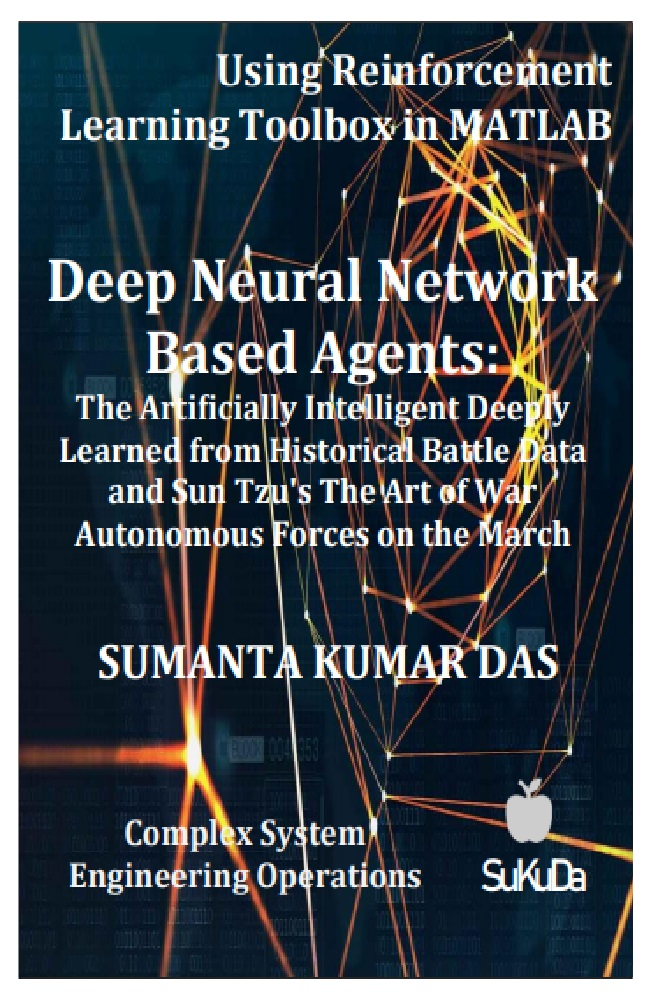
\includegraphics{front_cover1000by650.jpg}}
 \hspace*{-\textwidth}
 % \raisebox{3in}[0in][0in]{\color{black}
 % % \makebox[\textwidth][c]{\Huge Text over Image}
 % }
\
% \thispagestyle{empty}
% \addtocounter{page}{-1}%
%  \newpage
% % \RaggedLeft
%  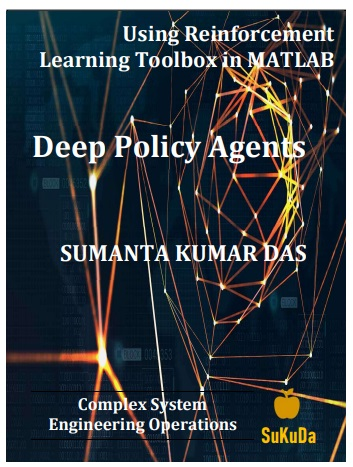
\includegraphics[width=\paperwidth,height=\paperheight]{deep_cover_front.jpg}

 \newgeometry{margin=0.4in,bottom=.4in}

% v.4 copyright page

 \newpage
 \centering
 \textbf{ \begin{Large}
       Deep Neural Network Based Agents:\end{Large} 
       \newline
 \begin{small}
 The Artificially Intelligent Deeply Learned from Historical Battle Data and Sun Tzu's The Art of War Autonomous Forces on the March \end{small} }
 \newpage
    \null
    \thispagestyle{empty}%
   \addtocounter{page}{-1}%
    \newpage
 
  \thispagestyle{empty}
 \pagenumbering{arabic}
\normalsize
 \section*{}
\thispagestyle{empty}
\begin{center}
 % \vspace*{.01cm}
    \normalsize
 
\textbf{ \begin{Large}
       Deep Neural Network Based Agents:\end{Large} 
       \newline
 \begin{small}
 The Artificially Intelligent Deeply Learned from Historical Battle Data and Sun Tzu's The Art of War Autonomous Forces on the March \end{small} }\\
\vspace{10mm}
Sumanta Kumar Das\\
% \newline
% \newline
% \newline
% \newline
% \newline
\vspace{20mm}
\small
SuKuDa\\
Self Publication\\
\thispagestyle{empty} 
\end{center}
 \tiny
% \begin{fullwidth}
% ~\vfill
\thispagestyle{empty}
% \setlength{\parindent}{0pt}
% \setlength{\parskip}{\baselineskip}
\centering
\vspace*{1mm}
\section*{}
\textbf{Deep Neural Network Based Agents: \\The Artificially Intelligent Deeply Learned from Historical Battle Data and Sun Tzu's The Art of War Autonomous Forces on the March }
\newline
\newline
\newline


Copyright \copyright\  \author{}{Sumanta Kumar Das}  \the\year\\
% P-ISBN: 978-93-5264-015-6\\
% E-ISBN: 978-93-5264-015-8\\
ISBN: 978-93-6128-100-6\\
% E-ISBN: xxx-xx-xxxx-xxx-x\\
% \justifying
\vspace{5mm}
\textbf{Published by}
\vspace{5mm}
\par\textbf{SuKuDa}

\par All rights are reserved and exclusively
Vested with the right-holder. No part of this work may be reproduced, stored, published, circulated, distributed, communicated, adopted, and translated in any material form (by electronic or mechanical means) without the prior written permission of the right-holder. Nothing herein prevents a person from making such uses that are permissible under law.\\
email:www.github/soomontodaas.com\\
website:www.mbsc.org\\
\vspace{5mm}

Second printing, 19 May 2024\\ Printed in India at\\ A5, Tower 10, Type 5\\East Kidwai Nagar,\\New Delhi-110023.


% \end{fullwidth}


\newpage
\RaggedRight
\section*{Chronology \cite{schmidhuber2022annotated}}
\normalsize
1676 Leibnitz, back rule \\
1800 Legendre, NN,  learning\\
1920 Ising, FNN, RNN\\
1927 Pavlop, Reinfor. Learning\\
1948 Turing Test\\
1958 Rosenblatt, MLNN\\
1965 Ivakhnenko, deep learning\\
1970 Linnainmaa, BackPropa\\
1972 Amari, First learning ANN\\
1979 First Deep Convolutional NN \\
1995 Neural Prob. Language Model\\
2015 DeepMind, \acrshort{dqn}, V. Mnih\\
2015 \acrshort{ddpg} Agent,Lillicrap\\
2017 \acrshort{ppo} Agent, J. Schulman\\
2018 \acrshort{sarsa}, Sutton R.S\\ 


\newpage
\pagestyle{fancy}
\fancyhead{}\fancyfoot{}
 % \fancyhead[C]{ \thepage}
\fancyfoot[C]{ \thepage}
\renewcommand{\headrulewidth}{0pt}
\renewcommand{\footrulewidth}{0pt}

\normalsize
\pagenumbering{roman}
\justifying{}
\section*{Forward}
\addcontentsline{toc}{section}{Foreword}
Data analysis by AI is a common thing nowadays. In the field of data analysis, many problems are being solved by machines by applying this technique.Especially Deep Learning technique has gained prominence in the time of now. Medical Science, Agriculture, and Bio-Informatics are the free movement of AI and Deep learning in all fields. In the field of combat modeling is no exception. Driven by this, UAVs, UGVs, and drones have now taken a special place in the era of Autonomous forces.To make these autonomous devices more sophisticated, they need to train more with historical battle data. As Human Soldier needs to be trained by Historical Battle Studies similarly Autonomous Robotic Forces need to be trained by historical data.This book is written very nicely to explain how battle data can be used for train the autonomous forces with the Sun Tzu's Art of War philosophy :\newline


Happy reading!\newline



\RaggedLeft    
Prof. Guang Yang\newline
ICL,London,UK\newline
Date:$3^{rd}$ \text{Feb,2024}
\newpage 
% \setcounter{page}
% \newpage

\normalsize
\section*{Preface}
\addcontentsline{toc}{section}{Preface}
\justifying
Recent times RL has gained significant popularity in simulating competitive games. The ability to reinforcement learned patterns through  deep artificial neural network is an essential components of an  intelligent force.:
\begin{enumerate}
    \item Deep learning is therefore an ideal choice of so called "Intelligent military robots" which involve processing and fusion of data from different sources and historical databases of differential equation\index{differential equation} based combat modeling\index{combat modeling} \Gls{combat modeling}.
    \item Advance level of \acrlong{ai} (\acrshort{ai}) based Model Fitting
    \item Introduction of simple theorems, Notations, and logic of combat modeling.
    \item The glossary and Acronyms of most useful terms of combat modeling.
\end{enumerate}
This book is a beginner’s introduction to \Gls{Artificial Intelligence} based model fitting for generating simple equations which can also be used in combat analysis, defence planning or even on in any battle analysis. The book does not attempt to compile all modeling techniques and algorithm available in the open literature it tries to present those models which suits best with combat analysis. The goal is to keep all important historical pattern setting battles in a common place which can be shared as graphical and network presentations in the defense analysis.
\newline
Happy reading!\newline


\RaggedLeft    
Sumanta Kumar Das\newline
New Delhi\newline
Date:$3^{rd}$ \text{Feb,2024}
\newpage
% \addtocounter{page}

\section*{Summary}
\addcontentsline{toc}{section}{Summary}
\justifying
Can \Gls{Autonomous Forces} be trained with Artificially Intelligence (AI) algorithms like \Gls{deep learning} from historical data and further be improved by the rules set by \Gls{Sun Tzu's Art of War} for developing a state-of-the-art system of planning and analysis of \Gls{Military Strategy}. The application of Machine learning (ML) algorithms are general practice for extracting meaningful models from the data. ML could be unsupervised, supervised, or reinforcement learning. This book explores deep learning neural networks for extracting model parameters for generating autonomous forces, Although our main focus is on the world's largest tank battle that is Battle of Kursk, we are also exploring other iconic historical battle data of the world for validating the system.  
The battle of Kursk between the Soviets and Germans is known to be the biggest tank battle in the history. This book explores the two-dimensional-simplex tank and artillery data from the Kursk database for analyzing a class of discrete time homogeneous and heterogeneous Lanchester models. Under homogeneous form, the Soviet’s (or German’s) tank casualty is attributed to only the German’s (or Soviet’s) tank engagement. For heterogeneous form, the tank casualty is attributed to both tank and artillery engagements. For validating the models, different goodness-of-fit statistics are used for comparison. 
\newpage
% \stepcounter{page}



% \section{Introduction}
% This is a test document which uses A4-sized paper and the user-defined text area. 
% \subsection{Some dummy text}
% \articletype{109^{th} ISC 3-5^{th} Jan 2024:Lovely Professional University,Punjab}% Specify the article type or omit as appropriate

% The emptypage package prevents page numbers and
% headings from appearing on empty pages.
% \thispagestyle{empty}
\tableofcontents
% \thispagestyle{empty}
\newpage
\scriptsize
% \thispagestyle{empty}
\listoffigures
% \thispagestyle{empty}
\newpage
\listoftables
% \thispagestyle{empty}
\newpage
 \thispagestyle{empty}
 \pagenumbering{arabic}
\normalsize
 \section*{}
\thispagestyle{empty}
\begin{center}
\thispagestyle{empty} 
% \vspace*{.01cm}
   \Large
 
\textbf{ Deep Neural Network Based Agents: \\The Artificially Intelligent Deeply Learned from Historical Battle Data and Sun Tzu's The Art of War Autonomous Forces on the March   }

\newpage

 
\small
% \author{
\textbf{Sumanta Kumar Das\footnote{phone:9811525928. Email: sumantadas.delhi@gmail.com} }\\
$SuKuDa^{TM}$ Self-Publication \\668 R.N. Tagore Road, P.O. Bediapara, Dumdum, \\
24 Pargonas(South), Kolkata-700077 \\
\end{center}
% \maketitle
\providecommand{\keywords}[1]{\textbf{\textit{Keywords---}} #1}

\begin{abstract}
Can autonomous forces\index{autonomous forces} be trained with \acrlong{ai} (\acrshort{ai}) algorithms like deep learning\index{learning} from historical data and further be improved by the rules set by Sun Tzu's Art of War for developing a state-of-the-art system of planning and analysis of military strategies? The application of \acrlong{ml} (\acrshort{ml}) algorithms are general practice for extracting meaningful models from the data. ML could be unsupervised\index{unsupervised}, supervised\index{supervised}, or reinforcement learning\index{learning!reinforcement learning}. This book explores deep learning neural networks for extracting model parameters for generating autonomous forces, Although our main focus is on multiple types of conflicts ranging from the world's largest tank battle that is the Battle of Kursk to the world's longest continuous military conflict that is the Battle of Atlantic, we are also exploring other historical battle data (Battle of Trafalgar,Iwo Jima, Ardennes and Britain ) of the world for validating the system.  
The battle of Kursk\index{Kursk} between the Soviets and Germans is known to be the biggest tank battle in history. This book explores the two-dimensional-simplex tank and artillery data from the Kursk database for analyzing a class of discrete time-homogeneous and heterogeneous Lanchester models. Under homogeneous form, the Soviet’s (or German’s) tank casualty is attributed to only the German’s (or Soviet’s) tank engagement. For heterogeneous form, the tank casualty is attributed to both tank and artillery engagements. Similarly, the Battle of Atlantic involves submarine, U-boat and Escort boat data for the same purpose. For validating the models, different goodness-of-fit statistics are used for comparison. 
\end{abstract}

\begin{keywords}
Battle of Kursk\index{Battle of Kursk}, Homogeneous\index{Lanchester's! Homogeneous Model} , Heterogeneous Lanchester Model\index{Lanchester's! Heterogeneous Model}, Goodness-of-Fit\index{Goodness-of-Fit},  Sum-of-Square Residuals\index{Sum-of-Square Residuals}, Chi-Square\index{Chi-Square}, Kolmogorov Smirnov\index{Kolmogorov-Smirnov}.
\end{keywords}
\newpage

% \chapter{Introduction}
% Chapter 1: A short chapter that ends on page 1.

\section{Introduction}
During the past decades, many differential equation based models \autocite{HelmboldRehm:1991,Lanchester:1916,Osipov:1915,Weiss:1975,Schramm:2012} have gained significant importance for representing combat dynamics. These equations are widely used for modelling in warfare and representing the decrease in force levels over time commonly referred to as attrition\index{attrition} process.Lanchester in 1914 proposed a set of differential equations, which quantify the importance of force concentration on the battlefield. Many authors have subsequently modified his original work to represent combat dynamics in modern warfare. In the recent time AI-enabled warfare involving "Killer Robots\index{Killer Robots}" \autocite{lethalRobots} has forced the designer to change the visualization of combat model development from traditional statistical methods to more practical adaptive\index{adaptive} and heuristic\index{heuristic} approaches. In \autocite{Davis2022ArtificialIF} the authors have discussed how artificial intelligence (AI) could be used in political-military modeling, simulation, and \\wargaming of conflicts with nations having weapons of mass destruction\index{weapons of mass destruction} and other high-end capabilities involving space, cyberspace, and long-range precision weapons. In reference \autocite{FATHM:2007}, we found that a fast large-scale theater model\index{theater model} combining ground to ground battle attrition with air-to-ground strikes has been developed using such models.The features of the Lanchester's Equation\index{Lanchester's ! Equation} that makes it suitable for analysis includes:
\begin{itemize}
  \item \textbf{\textit{Applicability}}:Lanchester models are widely used for historical battle analysis \autocite{Engel:1954}. Other than analysing human warfare Lanchester model have also been used for analysis of fights among social animals, market analysis \autocite{remnet:2016}.
  \item \textbf{\textit{Force Aggregation\index{Aggregation}}}: Lanchester models are found to be suitable for developing aggregated combat modelling using High Resolution Simulation Model\index{High Resolution Simulation Model}. In reality, actual historical combat data is not easily available and common practice is to develop High Resolution simulation data with detailed design. Various literature \autocite{Brackney:1959}, \autocite{Das:2007} \autocite{Das:2015} have demonstrated that estimating attrition rates from high-resolution simulation and using Lanchester model for linking the various resolution of different simulation model.
  \item \textbf{\textit{Flexibility}}: Lanchester models are flexible for both homogeneous as well as heterogeneous situations.Lanchester models are used for theoretically consistent force aggregation and \\dis-aggregation in two dimensions \autocite{Taylor:1983,Hillestad:1995}.
\end{itemize}
Regardless of credits of prior discovery, Lanchester's equations are used worldwide for calculating attrition rates. We propose an iterative parameter estimation algorithm for general form of the heterogeneous Lanchester's model as:
\begin{equation} 
%\begin{array}{}
      \Dot{X}_{i_{t}^{'}}=\sum_{i=1}^F a_{i}X_{i_{t}^{'}}^{q_{i}}Y_{i_{}^{'}}^{p_{i}}
%\end{array}
\end{equation}
\begin{equation}
%\begin{array}{}
     \Dot{Y}_{i_{t}^{'}}=\sum_{i=1}^F b_{i}Y_{i_{t}^{'}}^{q_{i}}X_{i_{}^{'}}^{p_{i}}\ ,\forall{i^{'}}=1,2,...F
%\end{array}
\end{equation}
where  $X_{{i}_{t}}$ denotes the strength of the $i$ th type of Red forces at time $t$ and  $Y_{{i}_{t}}$ denotes the strength of the $i$th type of Blue forces at time $t$. $\Dot{X_{{i}_{t}}}$ and $\Dot{Y_{{i}_{t}}}$ are red and blue forces killed at time $t$.

$a_{i}$ represents attrition rate of $i$th type of Blue forces and 

$b_{i}$ represents attrition rate of $i$th type of Red forces;

\(\forall{i}=1,2,...F\)

where 

\(F\) denotes the total number of forces. 

\(p_{i}\) the exponent parameter of the attacking force, 

\(q_{i}\) is the exponent parameter of the defending force. 


Equations (1) and (2) involve unknown parameters $a_{i}$,$b_{i}$ ,$p_{i}$ and \(q_{i}\). A lot of work has been done to estimate these parameters using statistical estimation\index{estimation} methods like Least Square\index{Least Square}, Maximum Likelihood\index{Maximum Likelihood}, Bayes\index{Bayes}, Method of Moments\index{Method of Moments} \autocite{Das:2007,Das:2015} etc. These estimates are most suitable for homogeneous situation. In heterogeneous situations these estimation procedures fail. In this book we propose AI based generalized reduced gradient\index{generalized reduced gradient} (\acrshort{grg}) algorithm \autocite{Hashemi2020PerformanceCO,Luo2022GeneralizedDL} which is alternatively solved through Deep learning Neural Network\index{Deep learning Neural Network}.  We are generally acquainted with two forms of these equations for homogeneous weapon engagement (when \(i\). Lanchester linear law in which \(p_{i}=q_{i}=1\) and force ratios remain equal if
\(a_{i}.X_{i_{0}^{}}^{p_{i}}=b_{i}.Y_{i_{0}^{}}^{q_{i}}\). Lanchester's linear law\index{Lanchester's!linear law} is interpreted as a model from a series of one-on-one duel between homogeneous forces and this law describes combat under "ancient conditions". The equation is also considered a good model for area fire weapons, such as artillery. Lanchester square law\index{Lanchester's!square law} in which , that is, force ratios remain equal if  applied to modern warfare in which both sides are able to aim their fire or concentrate forces.

On integrating equation (1) and (2) we obtain the state equation:
\begin{equation} 
%\begin{array}{}
      \frac{{\sum\limits_{i=1}^{X_{N}}}\sum\limits_{j=1}^{Y_{N}}{{a_{i}^j}{X_{i}.X_{j}}{{Y_{i}.Y_{j}}} }}{{\sum\limits_{i=1}^{X_{N}}}\sum\limits_{j=1}^{Y_{N}}{X_{i}^0.X_{j}^0}{{Y_{i}^0.Y_{j}^0}} }=1 
%\end{array}
\end{equation}
where ${X_{i}^0,X_{j}^0,Y_{i}^0,Y_{j}^0}$ , represent the initial values of Blue and Red forces respectively. This equation says that the relationship between the power of the losses in any fixed time period is equal to the inverse ratio of the attrition rate parameters. Equation (3) leads to the victory condition for Blue. Most forces have breakpoints at which they will cease fighting and either withdraw\index{withdraw} or surrender if:  
\begin{equation} 
%\begin{array}{}
      \frac{{\sum\limits_{i=1}^{X_{N}}}\sum\limits_{j=1}^{Y_{N}}{{a_{i}^j}{X_{i}.X_{j}}{{Y_{i}.Y_{j}}} }}{{\sum\limits_{i=1}^{X_{N}}}\sum\limits_{j=1}^{Y_{N}}{X_{i}^0.X_{j}^0}{{Y_{i}^0.Y_{j}^0}} }>1
%\end{array}
\end{equation}
Finally equations (4) may be solved in closed form as function of \textit{t}.
\begin{equation}
       X_{i}^{p_i}=\frac{1}{2}((X_{i_{0}}^{p_i}-Y_{i_{0}}^{q_i}\sqrt{\frac{a_{i}}{b_{i}}})e^{t\sqrt{a_i.b_i}}) 
       \nonumber
\end{equation}
\begin{equation}\\+\frac{1}{2}((X_{i_{0}}^{p_i}-Y_{i_{0}}^{q_i}\sqrt{\frac{a_{i}}{b_{i}}})e^{-t\sqrt{a_i.b_i}})
\end{equation}

\begin{equation}
       Y_{i}^{p_i}=\frac{1}{2}((Y_{i_{0}}^{p_i}-X_{i_{0}}^{q_i}\sqrt{\frac{a_{i}}{b_{i}}})e^{t\sqrt{a_i.b_i}}) 
       \nonumber
\end{equation}
\begin{equation}\\+\frac{1}{2}((Y_{i_{0}}^{p_i}-X_{i_{0}}^{q_i}\sqrt{\frac{a_{i}}{b_{i}}})e^{-t\sqrt{a_i.b_i}})
\end{equation}

There is another form of mixed combat model where attacker uses area fire (\begin{math}{{p_{i}=q_{i}=1}}\end{math} i.e. linear form) against a defender using aimed fire ( \begin{math}{p_{i}=1, q_{i}=0}\end{math} i.e. square form). This mixed form of combat model is known as ambush\index{ambush} model proposed by Deitchman \autocite{deitchman:1962lanchester}.

Helmbold \autocite{Helmbold1965LetterTT}in 1965 studied the Iwo-Jima campaign between USA and Japan using one-sided homogeneous Lanchester model. Bracken in 1995 studied Ardennes Campaign\index{Ardennes Campaign} between Germany and USA. Clemens in 1997 \autocite{Clemens:1997} and Lucas and Turkes in 2003 \autocite{LukasTurkes:2004} studied the Kursk campaign between Soviet and Germany. Willard \autocite{Willard1962LANCHESTERAF} has tested the capability of the Lanchester model for analyzing the historical battle data for the battles fought between the years of 1618-1905. 
Bracken\autocite{Bracken:1995} (1995) used the database of the Ardennes campaign of World War II formulating four different models which are the variations of the basic Lanchester equations. The models developed in his study were homogeneous in nature in terms of tank, \acrshort{apc}, artillery etc. He concluded that Lanchester linear model best fits the Ardennes campaign data in terms of minimizing the sum of squared residuals (\acrshort{ssr}). This work validates the applicability of the Lanchester model for the historical Battle data.
Fricker \autocite{Fricker:1998} revised the Bracken's models of the Ardennes campaign of World War II. He extended Bracken's model by applying linear regression on the logarithmic transformed Lanchester equations and included the data from the entire campaign and air sortie data as well. Lastly, he concluded that neither of the Lanchester linear or square laws fit the data. A new form of Lanchester equations emerges with a physical interpretation.

Clemens \autocite{Clemens:1997} fits the homogeneous version of Lanchester equations to the Battle of Kursk. He used two different techniques (i) Linear regression on logarithmic transformed equations (ii) a non-linear fit to the original equations using a numerical Newton-Raphson algorithm. 

Hartley and Helmbold \autocite{RePEc:wly:navres:v:42:y:1995:i:4:p:609-633} examined the validity of Lanchester's square law using the one-sided data from the Inchon-Seoul Campaign. They have not found good fit using constant coefficient square law but better fit was found when the data was divided into a set of three separate battles. They concluded the Lanchester's square law is not a proven attrition algorithm for warfare although they also commented that one-sided data is not sufficient to verify or validate Lanchester square law or any other attrition law. They have used linear regression, Akaike Info criterion and Bozdogan's consistency \acrshort{aic}(\acrshort{baic}). Based on the regression analysis they have found the models with three regression parameters with intercept and without intercept was the best model with higher degree Coefficients of determination.

NR Johnson and Mackey \autocite{JohsonMackey:2011}analysed the Battle of Britain using the Lanchester model. This was a battle of an air combat between German and Britain.

Wiper, Pettit and Young \autocite{WiperPetit:2000} applied Bayesian computational techniques to fit the Ardennes Campaign data. They studied stochastic form of Lanchester model and enquired whether there is role of any attacking and defending army on the number of casualties of the battle. They compared their results with the results of the Bracken and Fricker and results were found to be different. They concluded that logarithmic and linear-logarithmic forms fits more appropriately as compared to the linear form found by Bracken. They also concluded that the Bayesian approach is more appropriate to make inferences for battles in progress as it uses the prior information from experts or previous battles. They have applied the Gibbs sampling approach along with Monte Carlo simulation for deriving the distribution patterns of the parameters involved. 

Turkes \autocite{Turkes:2000} extended the previous work for the validation of Lanchester models with real data. He stated that historical data for validation of attrition model is poor. Mostly, the data contained starting sizes and casualties only for one side. He applied various derivatives of Lanchester equations for fitting model on the Kursk Database. The results found in his study were different with earlier studies on the Ardennes campaign. He found that wide variety of models fit the data as well. He has shown none of the basic Lanchester models fit the data, bringing into question their use in combat modelling. 
Lucas and Turkes \autocite{LukasTurkes:2004} used a new approach to find the optimal parameters for fitting Lanchester models on the data of Battles of Kursk and Ardennes. They have gained an understanding of how well various parameter combinations explain the battles. They have found that variety of models fits the data.They concluded that none of the basic laws (i.e. square, linear and logarithmic) fit the data correctly and raises the question of utility of basic Lanchester model for combat modelling. They also suggested finding new ways to model the aggregated attrition process to provide a good-fitting Lanchester model.

US Army’s Colonel Trevor N. Dupuy \autocite{dupuy1990evolution} discussed about different weapon system in his book about the Evolution of Weapons and Warfare (1990) which had evolved from 2000 BCE onwards till the Cold War and their tactical impact on combat. Despite its Western bias, the book is good for detailed description of the military hardware which modern Europe produced. Eminent author K Roy \autocite{Roy2022} described a global history of warfare from slings to drones also includes discussion on insurgency, civil war, sieges, skirmishes, ambushes and raids.
Petro \autocite{6928214} was introduced to develop multi-agent system for historical warfare which is useful for generating tactics of different kinds of military forces. It can be at soldier or at regimental level. Modeling of Various types of military forces namely Tatar riders, line infantry, Heussars, Reiters were introduced in this paper. 
Similarly WarAgent \autocite{hua2024war} is an example of \acrshort{llm} (\Gls{Large Language Model}) based \acrshort{mas} (\Gls{Multi Agent System}) for simulation of historical events.

	The main aim of this book is to fit Lanchester Model based on Kursk data.For that we require to estimate attrition rates and exponent parameters. There are several approaches to estimate the parameters. We shall consider two common and rational procedures namely, Least Square Estimation (\acrshort{lse}) and Maximum Likelihood Estimation (\acrshort{mle}). These two estimation procedures will be applied by AI techniques like Deep Learning. The authors in \autocite{lillicrap2019continuous} have demonstrated Deep Reinforcement Learning (\acrshort{drl}) AI techniques for solving complex problem, our autonomous forces are configured with this technique. DRL is an iterative optimization process. Our autonomous force higher commanders are established on the logic of \acrlong{ddpg} ($DDPGAgent$) \autocite{lillicrap2019continuous}. These\\ $DDPGAgents$ are represented by {actor-critic} relationship where Actor is $\pi($S$,\theta)$, for observations $S$ with parameter $\theta$ and critic $Q(\phi,$S$,$A$)$ with parameter, observation and action are $\phi$,$S$,$A$ respectively. The parameter $\theta$ is periodically updated for optimal value of long term reward function that produces the target Actor $\phi(S,\theta_t)$ and target critic $Q(\phi_t,$S$,$A$)$. In the present book the observations are historical battle data, actions are mathematical functions formulated from "Art of the War"\autocite{tzu2020art},the parameters $\theta$ estimated are attrition rate coefficients, exponents parameters which are being estimated through Deep Learning Neural Network, the critic parameters $\phi_t$ are estimated from the same data set with strategic inputs and rules from the "Art of the War". The long term reward function is designed from the GOF measures as defined in subsequent sections.
 The observations sets are Soviet's and German's Tank, APC, Arty Gun , Infantry. That is {1 * 8}, these datasets are discrete in nature. The actions are casualties in these components which is recorded as discrete elements. To create the discrete and continuous observation and action spaces for the \acrshort{rl}, \Gls{rlNumericSpace} and \Gls{rlFiniteSetSpace} are used.   

 

In the next section we have discussed in detail the mathematical formulations of homogeneous and heterogeneous situations. We have seen in Bracken \autocite{Bracken:1995}, Fricker \autocite{Fricker:1998} , Clemens \autocite{Clemens:1997} , Turkes\autocite{Turkes:2000}, Lucas \autocite{LukasTurkes:2004} that LSE method have been applied for evaluating the parameters for fitting the homogeneous Lanchester equations to the historical battle data.The MLE method \autocite{rohatgi2015introduction,Taylor:1983} has not been explored particularly for fitting the historical battle data till date. Also only one measure i.e. Sum-of-squared-residuals (SSR) has been explored for measuring the Goodness-of-fit (\acrshort{gof}). The main objective of this study is to assess the performance of the MLE approach for fitting homogeneous as well as heterogeneous Lanchester equations to the Battle of Kursk. Various measures of GOF \autocite{Agustino:1986} viz. \acrlong{ks}, \acrlong{chisquare} and $R^2$ have been computed for comparing the fits and to test how well the model fits the observed data. Applying the various GOF measures considering the artillery strength and casualties of Soviet and German sides from the Kursk battle data of World War-II validates the performance of MLE technique.\\Section 2 presents in brief the overview of the battle of Kursk. Section 3 describes the mathematical formulation of likelihood estimation in case of both homogeneous as well as heterogeneous situations. Section 4describes the Tank and Artillery data of Battle of Kursk and discusses the methodology for implementing the proposed as well as other approaches. Also, this section contains a performance appraisal of the MLE using various GOF measures. Section 5analyses the results after observing various tables and figures and discusses how well the MLE fits the data. Section 6 summarizes the important aspects of the book.
\newpage
\section{Iconic Battles}
The Battle of Trafalgar was a naval engagement that took place on 21 October 1805 between the British Royal Navy and the combined fleets of the French and Spanish Navies during the War of the Third Coalition (August–
December 1805) of the Napoleonic Wars (1803– 1815)\cite{BattleOfTrafalgar}.

The Battle of the Ardennes took place during the First World War fought on the frontiers of France, Germany, Belgium and Luxembourg from 21 to 23 August 1914. The German armies defeated the French and forced their retreat. 

The Battle of Britain (German: Luftschlacht um England, "air battle for England") was a military campaign of the Second World War, in which the Royal Air Force (RAF) and the Fleet Air Arm (FAA) of the Royal Navy defended the United Kingdom (UK) against large-scale attacks by Nazi Germany's air force, the Luftwaffe. It was the first major military campaign fought entirely by air forces\cite{BattleOfBritain}. The British officially recognise the battle's duration as being from 10 July until 31 October 1940, which overlaps the period of large-scale night attacks known as the Blitz, that lasted from 7 September 1940 to 11 May 1941\cite{BattleOfBritain2}. German historians do not follow this subdivision and regard the battle as a single campaign lasting from July 1940 to May 1941, including the Blitz\cite{overy2013bombing}.


The Battle of the Atlantic(naval Blockade), the longest continuous military campaign in World War II, ran from 1939 to the defeat of Nazi Germany in 1945, covering a major part of the naval history of World War II\cite{blair2010hitler},\cite{woodman2011real}.

After suffering a terrible defeat (\Gls{Withdrawal},) at Stalingrad in the winter of 1943, the Germans desperately wanted to regain the initiative. In the spring of 1943, the Eastern front was conquered (\Gls{Breakthrough}) by a salient, 200 km wide and 150 km deep, centred on the city of Kursk. The Germans planned in a classic pincer operation named Operation Citadel, to eliminate the salient and destroy the Soviet forces (\Gls{Prepared Defense}) in it. On 2 July 1943, Hitler declared, "This attack is of decisive importance and it must succeed, and it must do so rapidly and convincingly. It must secure for us the initiative.... The victory of Kursk must be a blazing torch to the world" \autocite{JohsonMackey:2011,Klug:2003,Wiki}.

The Germans started the Battle of Kursk on July 4, 1943 on the southern half of the Kursk salient, but this was merely to gain better artillery observation points(\Gls{Hasty Defense}). The battle began in earnest early in the morning of July 5, when Soviets conducted an artillery barrage before the 
Wehrmacht attacked. The Germans countered with their own planned barrages shortly thereafter 
and seized the initiative on both fronts. Soviet General Rokossovsky redeployed his reserves on 
the night of July 5 in order to attack the following day. The divisions of the 17th and 18th Guards 
Rifle Corps, with support from the 3rd, 9th, 16th, and 19th Tank Corps, were beginning offensive operations at 5:30 a.m. on July 6 in support of 13th Army. July 6 were considered as worst single day of CITADEL for German tank losses.On 7th July the German attack with armour forces in the northern and northeast side and captured the village Lutschki and continued advancing towards the village of Tetrevino against the very strong Soviet infantry and armor battle. By evening July 7 the Germans were ableto capture the village Tetrevino. On 8th July the German attacked with armour forces and barely captured the Teploye village. The Soviet counterattacked and recapture the lost Teploye village.The soviet defended very well on that day although they lost 315 tanks on that day in comparison to 108 tank loss of the Germans. The German forces wanted to develop a sharp wedge towards Kursk via Oboyan village. The German forces attacked with more than 500 tanks.The soviet forces defended the Oboyan with sophisticated artillery guns. Despite the strong defense the Germans were able to foothold over the Pena River. During the period of July 7-9both the sides had suffered largest number of tank losses. Due to this reason the Germans planned to attack from less resistance Prokorovka side. After changing the direction of the attack the German reached and seized the village of Novoselovka. The Soviets understood the German's plan and they started using their reserve units. But despite of that the Germans were able to break through (\Gls{Breakthrough}) the Soviet defenses by evening of the July 10. The German intention at this point was to cross the river Psel to the extent of as many as troops and vehicles are possible. The Germans were able to seize a bridge. The engagement was at this point between artillery and tank.Both the forces were preparing for the battle of Prokhorovka. \\
The Battle of Prokhorovka was the decisive phase of the Battle of Kursk. The Soviets started with artillery defense and later it turns out to be totally tank against tank meeting engagement (\Gls{Meeting Engagement},). The German tanks had to face minefield as well as well defended Soviet anti-tank weapons\Gls{Delaying}, (\Gls{Delaying},). The resulting titanic battle was a tactical draw (\Gls{Stalemate},). The Germans lost 98 tanks against 414 Soviet tank losses. Hitler called off the battle. The losses from the fighting over July 12 and 13 were extensive on both sides. In KUTUZOV there was a heavy armour engagement between the two forces. The German forces destroyed 117 Soviet tanks. The Soviets also damaged 57 German tanks.The battle on Prokorovka still continued on 14th July. The German planned an offensive operation named operation Roland. It started on July 14. The aim was to destroy the Soviet armor reservoirs\\(\Gls{Deliberate Defense}). The German armor units fought with the artillery forces that were defending the armor reservoirs of the Soviet in the southern part of the Prokorovka. Several tactical positions\\ (\Gls{Fortified Defense}) were captured by the German forces. On this day the Germans were capable of performing minor offensive operations and they were launching attacks to form the Gostishchevo-Liski pocket. Hitler redirected it back to Isyum on July 16. According to the various war analysts it is being considered that because of Hitler's decision, von Manstein lost the availability of a powerful mobile formation that could have been very useful in the battle. During this time most of the engagements were between German infantry and Soviet tanks. Most of the damage was suffered by the Soviet because they were not equipped with modern antitank weapons that can deal effectively with the Soviet armour. The Soviets launched their counteroffensive along the Mius River on July 17. The Southwestern Front, commanded by Colonel General Tolbukhin, attacked the heavily fortified Mius River line defenses(\Gls{Fortified Defense}). The Soviet counter attack was known as operation RUMANTSYEV.

The Battle of Iwo Jima (19 February – 26 March 1945) was a major battle in which the United States Marine Corps (USMC) and United States Navy (USN) landed on and eventually captured the island (fortified defence) of Iwo Jima from the Imperial Japanese Army (IJA) during World War II. The American invasion, designated Operation Detachment, had the purpose of capturing the island with its two airfields: South Field and Central Field\cite{BattleOfIJ}.

% The \Gls{latex} typesetting markup language is specially suitable 
% for documents that include \gls{maths}. \Glspl{formula} are 
% rendered properly an easily once one gets used to the commands.
% Given a set of numbers, there are elementary methods to compute 
% its \acrlong{gcd}, which is abbreviated \acrshort{gcd}. This 
% process is similar to that used for the \acrfull{lcm}.

\clearpage
\newpage
\section{Estimation}
Let $S$ denote the time between two consecutive casualties for a side, its probability density function is denoted by $f_S(S)$. Let $({m_k}^i,{n_k}^i)$  represents the ${i}^{th}$ type force strengths (e.g. tank, artillery etc.) of blue and red forces of a battle for the ${k}^{th}$ time instance respectively. Let us also denote (for $k=1,2\dots K$) the time (a random variable) at which $K^{th}$ casualty occurs on $T_k$ (with realization $t_k$). Let the Blue and Red casualties $\Dot{X}_{i'_t}$ and $\Dot{Y}_{i'_t}$  in a combat are r.v. whose densities are defined by $f_{s_X}(s | a_i,p_i,q_i)$  and  $f_{s_Y}(s | b_i,p_i,q_i)$ respectively where forms of the densities are known except the unknown parameters \\$(a_i,b_i,p_i,q_i)$.It is assumed that the   of a random sample  ($\Dot{x}_{i'_t}$,$\Dot{y}_{i'_t}$)from $f_S(S)$ can be observed. On the basis of the observed sample values ($\Dot{x}_{i'_t}$,$\Dot{y}_{i'_t}$) it is desired to estimate the value of the unknown parameters $(a_i,b_i,p_i,q_i)$ . We further assume that the times between casualties are exponentially distributed, then the pdf  of casualty for the Red ($X$) and Blue ($Y$) sides associated to the equation (1) and (2) can be represented as in the equations  and :
\begin{multline*}
     f_{S_{{x}_{i^{'}}}}(s)=
     {\prod_{i=1}^{F}}(a_i.{x_{i'_t}}^{p_i}.{y_{i'_t}}^{q_i}).
     \\exp(-{(\sum_{i=1}^{F}a_i.{x_{i'_t}}^{p_i}.{y_{i'_t}}^{q_i})s)} \nonumber
     \end{multline*}
\begin{equation}\label{e3}
    -\infty<a_i,p_i,q_i<\infty,  \forall{i^{'}=1,2,\dots,F}
\end{equation}
\begin{multline*}\label{e4}
     f_{S_{{y}_{i^{'}}}}(s)=
     {\prod_{i=1}^{F}}(b_i.{x_{i'_t}}^{q_i}.{y_{i'_t}}^{p_i}).
     \\exp(-{(\sum_{i=1}^{F}b_i.{x_{i'_t}}^{q_i}.{y_{i'_t}}^{p_i})s)} \nonumber
     \end{multline*}
\begin{equation}\label{e5}
    -\infty<b_i,p_i,q_i<\infty,  \forall{i^{'}=1,2,\dots,F}
\end{equation}
The likelihood equation of $n$ pairs of random variable ($\Dot{x}_{i'_t}$,$\Dot{y}_{i'_t}$) is defined as the joint density of the n pairs of random variables, which is considered to be a function of $(a_i,b_i,p_i,q_i)$. In particular, if ($\Dot{x}_{i'_t}$,$\Dot{y}_{i'_t}$) are independently and identically distributed random sample from the density $f_S(S)$, then the likelihood function is:  
 
\begin{multline*}
f({{x_{i_{1}^{'}}}|a_i,p_i,q_i}).f({{y_{i_{1}^{'}}}|b_i,p_i,q_i}){\dots}\\f({{x_{i_{t}^{'}}}|a_i,p_i,q_i}).f({{y_{i_{t}^{'}}}|b_i,p_i,q_i})
    \end{multline*}
Then, the joint pdf will be:
\begin{multline*}\label{e7}
     L(a_i,b_i,p_i,q_i)=
     {\prod_{i=1}^{F}}{\prod_{i=1}^{F}}\\(a_i.{x_{i'_t}}^{p_i}{y_{i'_t}}^{q_i})^{\Dot{x}_{i'_t}}\\{\times}(b_i.{y_{i'_t}}^{p_i}.{x_{i'_t}}^{q_i})^{\Dot{y}_{i'_t}}{\times}
      \nonumber
\end{multline*}
\begin{equation}
    exp(-(\sum_{i=1}^{F}a_i.{x_{i'_t}}^{p_i}.{y_{i'_t}}^{q_i}+
    \nonumber
\end{equation}
\begin{equation}
   b_i.{y_{i'_t}}^{p_i}.{x_{i'_t}}^{q_i})s)
\end{equation}
    
To construct the likelihood function from the available data set, it is generally observed that casualty figures are generally available at daily interval. Let $L(a_i,b_i,p_i,q_i)$ be the likelihood function for the random variables ($\Dot{x}_{i'_t}$,$\Dot{y}_{i'_t}$). If $\hat{a}_i$, $\hat{b}_i$, $\hat{p}_i$, $\hat{q}_i$ are the values of  $a_i,b_i,p_i,q_i$ which maximizes $L(a_i,b_i,p_i,q_i)$ , then  $\hat{a}_i$, $\hat{b}_i$, $\hat{p}_i$, $\hat{q}_i$ are the maximum-likelihood estimates of  $a_i,b_i,p_i,q_i$. Now, instead of maximizing the likelihood function we will maximize its logarithmic form since both the maximum values occur at the same point and logarithmic form is easily imputable.
Thus, on taking log of equation (8), we have
\begin{equation}
     lnL=
     ({\prod_{i=1}^{F}}{\prod_{t=1}^{N}}{\Dot{x}_{i'_t}}ln(a_i.{x_{i'_t}}^{p_i}{y_{i'_t}}^{q_i})+
     \nonumber
\end{equation}
\begin{equation}
     \\  {\Dot{y}_{i'_t}}ln(b_i.{x_{i'_t}}^{q_i}{y_{i'_t}}^{p_i}))-{(a_i.{x_{i'_t}}^{p_i}.{y_{i'_t}}^{q_i}+}
     \nonumber
\end{equation}
\begin{equation}
     \\b_i.{y_{i'_t}}^{p_i}.{x_{i'_t}}^{q_i})s
\end{equation}
Differentiating the Log-likelihood function (9) partially with respect to $a_i$ and $b_i$ and equating it to zero, we have:
\begin{equation}
    \frac{dlnL}{da_i}=\sum_{t=1}^{N}{\frac{\Dot{x}_{i'_t}}{a_i}}-
    \nonumber
\end{equation}
\begin{equation}
    \sum_{i=1}^{F}\sum_{t=1}^{N}{y_{i'_t}}^{p_i}.{x_{i'_t}}^{q_i}s=0
\end{equation}
and
   \begin{equation}
    \frac{dlnL}{db_i}=\sum_{t=1}^{N}{\frac{\Dot{y}_{i'_t}}{b_i}}-
    \nonumber
\end{equation}
   \begin{equation}
    \sum_{i=1}^{F}\sum_{t=1}^{N}{x_{i'_t}}^{p_i}.{y_{i'_t}}^{q_i}s=0
\end{equation}
This gives
\begin{equation}
   \sum_{t=1}^{N}{\frac{\Dot{x}_{i'_t}}{a_i}}=\sum_{i=1}^{F}\sum_{t=1}^{N}{x_{i'_t}}^{p_i}.{y_{i'_t}}^{q_i}
\end{equation}
 and                             
 \begin{equation}
   \sum_{t=1}^{N}{\frac{\Dot{y}_{i'_t}}{b_i}}=\sum_{i=1}^{F}\sum_{t=1}^{N}{y_{i'_t}}^{p_i}.{x_{i'_t}}^{q_i}
\end{equation}
Thus, the maximum likelihood estimates are: 
\begin{equation}
\hat{a}_i=\frac{\sum_{t=1}^{N}{\Dot{x}_{i'_t}}}{\sum_{i=1}^{F}\sum_{t=1}^{N}{x_{i'_t}}^{p_i}.{y_{i'_t}}^{q_i}s}
\end{equation}
\begin{equation}
\hat{b}_i=\frac{\sum_{t=1}^{N}{\Dot{y}_{i'_t}}}{\sum_{i=1}^{F}\sum_{t=1}^{N}{y_{i'_t}}^{p_i}.{x_{i'_t}}^{q_i}s}
\end{equation}
\newpage
\section{Data}
The Kursk Data Base (\acrshort{kdb}) is developed by Dupuy Institute (DPI) and is reformatted into a computerized database in1998. KDB is documented in the KOSAVE (Kursk Operation Simulation and Validation Exercise) \autocite{KOSAVEII:1998}. The KDB contains daily on hand and losses for the four categories viz. manpower, tanks, APC and artillery for the Soviets and Germans for each of the 15 days of battle. Evidences of multiple force interaction in Kursk Battle shows multiple forces were fighting in the war. Therefore, developing heterogeneous model on this data is justified. In the present study, we have considered only the tank and artillery data for developing heterogeneous Lanchester model. Table 1 shows the tank and artillery weapons on hand and losses during the 14 days of battle. Figure 1 shows a comparison between the Soviet and German's tank losses during the 14 days of battle.

% \setcounter{table}{1}
% \footnotesize
\begin{sidewaystable}
 \centering

\tiny
\caption{Battle of Iwo Jima\\}
\vspace{0.5 cm}
\tiny

% \caption{Long table caption.\label{long}}
{\begin{tabular}{|p{.5cm}|p{.5cm}|p{.5cm}|p{.5cm}|p{.5cm}|p{.5cm}|p{.5cm}|p{.5cm}|p{.5cm}|} 
\hline
\centering
% Days & Soviet's Tank On Hand & Soviet's Tank Losses	& German's Tank On Hand	& German's Tank Losses & Soviet's Arty 
% On Hand	& Soviet's Arty Losses & German's Arty 
% On Hand	& German's Arty Losses \\

$Time$ & $USA$ & $JAP$	& $Time$	& $USA$ & $JAP$	& $Time$ & $USA$	& $JAP$ \\
\hline  	
0&0&21500&13&59549&NA&25&53347&NA\\
\hline
1&	52839&	NA	&14	&59345&	NA&	26	&53072&	NA\\
\hline
2&	50945&	NA	&15&	59081&	NA&	27&	52804&	NA\\
\hline
4&	56031&	NA&	16&	58779	&NA	&28	&52735	&NA\\
\hline
5&	53749&	NA	&17&	58196&	NA&	29&	52608&	NA\\
\hline
6&	66155&	NA&	18&	57259	&NA&	30&	52507&	NA\\
\hline
7&	65250&	NA&	19&	56641&	NA&	31&	52462&	NA\\
\hline
8&	64378&	NA&	20&	54792&	NA&	32&	52304&	NA\\
\hline
9&	62874&	NA&	21&	55308&	NA&	33&	52155&	NA\\
\hline
10&	62339&	NA&	22&	54796&	NA&	34&	52155&	NA\\
\hline
11&	61405&	NA&	23&	54038&	NA&	35&	52155&	NA\\
\hline
12&	60667&	NA&	24&	53938&	NA&	36&	52140&	0\\
\hline

% \hline
\end{tabular}}%\label{landtab}
\tiny
% {\footnote{$^1$\text{Days},$^2$\text{German's Tank On Hand},$^3$\text{German's Tank On Hand},\\$^4$\text{German's Tank On Hand},$^5$\text{German's Tank Casualty},\\$^6$\text{Soviet's Arty On Hand},$^7$\text{Soviet's Arty On Hand},\\$^8$\text{German's Arty On Hand},$^9$\text{German's Arty Casualty}}}\\
\end{sidewaystable}

\begin{table}


\tiny
\caption{Battle of Atlantic(U-boats losses \cite{hughes1977battle})\\}
\vspace{0.5cm}
\tiny

% \caption{Long table caption.\label{long}}
{\begin{tabular}{|p{.5cm}|p{.5cm}|p{.5cm}|p{.5cm}|p{.5cm}|p{.5cm}|} 
\hline
\centering
% Days & Soviet's Tank On Hand & Soviet's Tank Losses	& German's Tank On Hand	& German's Tank Losses & Soviet's Arty 
% On Hand	& Soviet's Arty Losses & German's Arty 
% On Hand	& German's Arty Losses \\

$Year$ & $Total$ & $Opral$	& $Eng$	& $Sunk$ & $New$ \\
\hline  
1939&	57&	12&	5&	9&	2\\
1940&	51&	11&	5&	6&	4\\
1940&	49&	10&	7&	8&	9\\
1940&	56&	10&	8&	5&	15\\
1940&	75&	11&	9&	3&	26\\
1941&	102&	20&	12&	5&	31\\
1941&	136&	25&	15&	7&	53\\
1941&	182&	30&	17&	6&	70\\
1941&	233&	35&	16&	17&	70\\
1942&	272&	45&	13&	11&	49\\
1942&	315&	60&	15&	10&	58\\
1942&	352&	95&	25&	32&	61\\
1942&	382&	100&	40&	34&	70\\
1943&	418&	110&	50&	40&	70\\
1943&	424&	90&	40&	73&	69\\
1943&	408&	60&	20&	71&	68\\
1943&	425&	70&	25&	53&	83\\
1944&	445&	65&	30&	60&	62\\
1944&	437&	50&	20&	68&	53\\
1944&	396&	40&	15&	79&	50\\
1944&	398&	35&	20&	32&	67\\
1945&	349&	45&	20&	153&	93\\

\hline

% \hline
\end{tabular}}%\label{landtab}
\tiny
% {\footnote{$^1$\text{Days},$^2$\text{German's Tank On Hand},$^3$\text{German's Tank On Hand},\\$^4$\text{German's Tank On Hand},$^5$\text{German's Tank Casualty},\\$^6$\text{Soviet's Arty On Hand},$^7$\text{Soviet's Arty On Hand},\\$^8$\text{German's Arty On Hand},$^9$\text{German's Arty Casualty}}}\\
\end{table}
\begin{table}
 

\tiny
\caption{Battle of Britain \cite{JohsonMackey:2011})\\}
\vspace{0.5cm}
\tiny

% \caption{Long table caption.\label{long}}
{\begin{tabular}{|p{.5cm}|p{.5cm}|p{.5cm}|p{.5cm}|p{.5cm}|p{.5cm}|} 
\hline
\centering
% Days & Soviet's Tank On Hand & Soviet's Tank Losses	& German's Tank On Hand	& German's Tank Losses & Soviet's Arty 
% On Hand	& Soviet's Arty Losses & German's Arty 
% On Hand	& German's Arty Losses \\

$Point$ & $\delta$G & $\delta$B	& G	& B & r \\
\hline  
1939&	57&	12&	5&	9&	2\\
1940&	51&	11&	5&	6&	4\\
1940&	49&	10&	7&	8&	9\\
1940&	56&	10&	8&	5&	15\\
1940&	75&	11&	9&	3&	26\\
1941&	102&	20&	12&	5&	31\\
1941&	136&	25&	15&	7&	53\\
1941&	182&	30&	17&	6&	70\\
1941&	233&	35&	16&	17&	70\\
1942&	272&	45&	13&	11&	49\\
1942&	315&	60&	15&	10&	58\\
1942&	352&	95&	25&	32&	61\\
1942&	382&	100&	40&	34&	70\\
1943&	418&	110&	50&	40&	70\\
1943&	424&	90&	40&	73&	69\\
1943&	408&	60&	20&	71&	68\\
1943&	425&	70&	25&	53&	83\\
1944&	445&	65&	30&	60&	62\\
1944&	437&	50&	20&	68&	53\\
1944&	396&	40&	15&	79&	50\\
1944&	398&	35&	20&	32&	67\\
1945&	349&	45&	20&	153&	93\\

\hline

% \hline
\end{tabular}}%\label{landtab}
\tiny
% {\footnote{$^1$\text{Days},$^2$\text{German's Tank On Hand},$^3$\text{German's Tank On Hand},\\$^4$\text{German's Tank On Hand},$^5$\text{German's Tank Casualty},\\$^6$\text{Soviet's Arty On Hand},$^7$\text{Soviet's Arty On Hand},\\$^8$\text{German's Arty On Hand},$^9$\text{German's Arty Casualty}}}\\
\end{table}

\begin{table}
 

\tiny
\caption{Battle of Ardennes \cite{JohsonMackey:2011})\\}
\vspace{0.5cm}
\tiny

% \caption{Long table caption.\label{long}}
{\begin{tabular}{|p{.5cm}|p{.5cm}|p{.5cm}|p{.5cm}|p{.5cm}|p{.5cm}|} 
\hline
\centering
% Days & Soviet's Tank On Hand & Soviet's Tank Losses	& German's Tank On Hand	& German's Tank Losses & Soviet's Arty 
% On Hand	& Soviet's Arty Losses & German's Arty 
% On Hand	& German's Arty Losses \\

$Point$ & $\delta$G & $\delta$A	& G	& A & r \\
\hline  
1939&	57&	12&	5&	9&	2\\
1940&	51&	11&	5&	6&	4\\
1940&	49&	10&	7&	8&	9\\
1940&	56&	10&	8&	5&	15\\
1940&	75&	11&	9&	3&	26\\
1941&	102&	20&	12&	5&	31\\
1941&	136&	25&	15&	7&	53\\
1941&	182&	30&	17&	6&	70\\
1941&	233&	35&	16&	17&	70\\
1942&	272&	45&	13&	11&	49\\
1942&	315&	60&	15&	10&	58\\
1942&	352&	95&	25&	32&	61\\
1942&	382&	100&	40&	34&	70\\
1943&	418&	110&	50&	40&	70\\
1943&	424&	90&	40&	73&	69\\
1943&	408&	60&	20&	71&	68\\
1943&	425&	70&	25&	53&	83\\
1944&	445&	65&	30&	60&	62\\
1944&	437&	50&	20&	68&	53\\
1944&	396&	40&	15&	79&	50\\
1944&	398&	35&	20&	32&	67\\
1945&	349&	45&	20&	153&	93\\

\hline

% \hline
\end{tabular}}%\label{landtab}
\tiny
% {\footnote{$^1$\text{Days},$^2$\text{German's Tank On Hand},$^3$\text{German's Tank On Hand},\\$^4$\text{German's Tank On Hand},$^5$\text{German's Tank Casualty},\\$^6$\text{Soviet's Arty On Hand},$^7$\text{Soviet's Arty On Hand},\\$^8$\text{German's Arty On Hand},$^9$\text{German's Arty Casualty}}}\\
\end{table}

\begin{sidewaystable}
\centering
 \tiny
\caption{Battle of Trafalgar\\}
\vspace{0.1cm}
\tiny

% \caption{Long table caption.\label{long}}
{\begin{tabular}{|p{.3cm}|p{.3cm}|p{.3cm}|p{.3cm}|p{.3cm}|p{.3cm}|p{.3cm}|p{.3cm}|p{.3cm}|p{.5cm}|} 
\hline
\centering
% Days & Soviet's Tank On Hand & Soviet's Tank Losses	& German's Tank On Hand	& German's Tank Losses & Soviet's Arty 
% On Hand	& Soviet's Arty Losses & German's Arty 
% On Hand	& German's Arty Losses \\

$B$ & $F$ & $S$	& $B$	& $F$ & $S$	& $B$ & $F$	& $S$ &$Win$ \\
\hline  	

4&	17&	16	&23	&17&	18&	18	&16&	11& British\\
5&	17&	16	&22	&17&	16&	16	&16&	8& British\\
6&	17&	16	&21	&17&	15&	15	&16&	6& British\\
7&	17&	15	&20	&17&	14&	14	&15&	5& British\\
8&	17&	14	&19	&17&	12&	12	&14&	2& France\\
9&	17&	13	&18	&17&	10&	10	&13&	6& France\\

\hline

% \hline
\end{tabular}}%\label{landtab}
\tiny
% {\footnote{$^1$\text{Days},$^2$\text{German's Tank On Hand},$^3$\text{German's Tank On Hand},\\$^4$\text{German's Tank On Hand},$^5$\text{German's Tank Casualty},\\$^6$\text{Soviet's Arty On Hand},$^7$\text{Soviet's Arty On Hand},\\$^8$\text{German's Arty On Hand},$^9$\text{German's Arty Casualty}}}\\
\end{sidewaystable}



\begin{sidewaystable}
 
\centering
\tiny
\caption{Daily Soviet and Germans on hand and losses data for tanks and artillery from Kursk Battle}
\tiny

% \caption{Long table caption.\label{long}}
{\begin{tabular}{|p{.1cm}|p{.5cm}|p{.3cm}|p{.3cm}|p{.3cm}|p{.3cm}|p{.2cm}|p{.4cm}|p{.2cm}|} 
\hline
\centering
% Days & Soviet's Tank On Hand & Soviet's Tank Losses	& German's Tank On Hand	& German's Tank Losses & Soviet's Arty 
% On Hand	& Soviet's Arty Losses & German's Arty 
% On Hand	& German's Arty Losses \\

$A^1$ & $B^2$ & $C^3$	& $D^4$	& $E^5$ & $F^6$	& $G^7$ & $H^8$	& $I^9$ \\
\hline
1&2396&105&986&198&705&13&1166&24\\
\hline
2&2367&117&749&248&676&30&1161&5\\
\hline
3&2064&259&673&121&661&15&1154&7\\
\hline
4&17546&315&596&108&648&14&1213&13\\
\hline
5&1495&289&490&139&640&9&1210&6\\
\hline
6&1406&157&548&36&629&13&1199&12\\
\hline
7&1351&135&563&63&628&7&1206&15\\
\hline
8&977&414&500&98&613&16&1194&12\\
\hline
9&978&117&495&57&606&10&1187&7\\
\hline
10&907&118&480&46&603&5&1184&5\\
\hline
11&883&96&426&79&601&5&1183&3\\
\hline
12&985&27&495&23&600&3&1179&4\\
\hline
13&978&42&557&7&602&0&1182&2\\
\hline
14&948&105&986&198&705&13&1166&24\\
\hline
% \hline
\end{tabular}}%\label{landtab}
\tiny
{\footnote{$^1$\text{Days},$^2$\text{German's Tank On Hand},$^3$\text{German's Tank On Hand},\\$^4$\text{German's Tank On Hand},$^5$\text{German's Tank Casualty},\\$^6$\text{Soviet's Arty On Hand},$^7$\text{Soviet's Arty On Hand},\\$^8$\text{German's Arty On Hand},$^9$\text{German's Arty Casualty}}}\\
\end{sidewaystable}

% \end{table}
\medskip

\begin{figure}
\centering
  % El fichero es un eps y se convierte automaticamente a pdf con eps2pdf package
  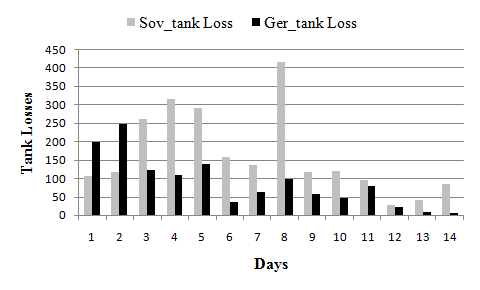
\includegraphics[width=4cm]{figure3.eps.png}\\
  \caption{Comparison of daily number of tank losses of the Battle of Kursk of WW II.}
\end{figure}
This book fits the generalized form of Heterogeneous Lanchester equations to the Battle of Kursk data using the method of Maximum Likelihood estimation and compares the performance of MLE with the techniques studied earlier such as the Sum of squared residuals (\acrshort{ssr}), Linear regression and Newton-Raphson iteration.Different authors applied different methodologies for fitting Lanchester equations to the different battle data. The methodologies of Bracken, Fricker, and Clemen are applied to the Tank data of Battle of Kursk and results are shown in Table 3.

The Battle of Atlantic Database\gls{Battle of Atlantic}
1. Merchant Ships
2. U Boat
3. Submarines
4. Date:September 3, 1939 – May 8, 1945 (5 years, 8 months and 5 days)
5. Allied(UK+USA) vs. Germany +Italy
6. Allied Losses: 36,200 killed (naval), 36,000 killed (merchant navy),
3,500 merchant vessels, 175 warships ,741 RAF Coastal Command aircraft lost in anti-submarine sorties.\cite{WikiBattleOfAtlantic}
\newpage
\section{Goodness-of-fit \\Statistics}
First, we applied the technique of Least Square for estimating the parameters of the heterogeneous Lanchester model. The GRG algorithm \autocite{Excel,MATLAB} is applied for maximizing the MLE and for minimizing the LSE. For implementing the Least Square approach, the Sum of Squared Residuals (SSR) is minimized. The expression of SSR for the equation (1) and (2) is given as: 
\begin{equation}
    SSR=\sum_{t=1}^{14}{(\Dot{x}_{i^{'}_t}-\sum_{i=1}^{2}a_i{x_{i^{'}_t}}^{p_i}{y_{i^{'}_t}}^{q_i})^2}+ \nonumber
\end{equation}
\begin{equation}
    \sum_{t=1}^{14}{(\Dot{y}_{i^{'}_t}-\sum_{i=1}^{2}b_i{y_{i^{'}_t}}^{p_i}{x_{i^{'}_t}}^{q_i})^2.}
\end{equation}                                    
For implementing this expression from table 1 we have taken zero as initial values for all the unknown parameters. Then we start running the GRG algorithm iteratively. The GRG algorithm is available with the Microsoft Office Excel (2007) Solver \autocite{Excel} and MATLAB \autocite{MATLAB}. The GRG solver uses iterative numerical method. The derivatives (and Gradients) play a crucial role in GRG.We have run the program for 1000 iterations for getting the stabilized values of these parameters. Once, we have the parameters we compute the estimated casualties. With the difference between the estimated and observed casualties, we computed the Sum of Squared Residuals. Similarly, we applied the GRG algorithm for optimizing the objective function as given in equation (9).We check the graphs of estimated and observed casualties for both the LS and MLE based approaches and found that if we divide the data set into several subsets then we can improve the fit. As we increase the number of divisions,the fit turns out to be better. The estimated casualty converges to the observed casualty. We have considered tank and artillery data for mixing the forces therefor ea1(or b1) represents effectiveness of Soviet(or Germans) tanks against Germans(or Soviets) tanks and a2(or b2) represents effectiveness of Soviets (or Germans)Arty against Germans (or Soviets) tanks.The variation of attrition rates throughout battle tells us how the different player in the battle performs. Whether they are acting defensively or offensively.

The basic idea of using GRG algorithm is to quickly find optimal parameters that maximize the \\log-likelihood.The objective is to find the parameters that maximize the log-likelihood or in other words provide the best fit. Given the values in Table 1, we investigate what values of the parameters best fit the data. Although we derived the estimates fora and b using the MLE approach in equations (8) and (9), they are not applied directly. Log Likelihood is calculated using the equation (7) considering 0.5 as the initial value of the parameters. Then, we optimized the entire duration of the battle of the likelihood function using the GRG algorithm.The model obtained after estimation of parameters is:
\begin{equation}
\begin{split}
    \Dot{x}_1=&(1.46){x_1}^{.129}{y_1}^{.404} \\
     &+(.906){x_1}^{.138}{y_2}^{.136} \\
     \Dot{y}_1=&(.704){y_1}^{.129}{x_1}^{.404}\\
      &+(.953){y_1}^{.138}{x_2}^{.136}\\
\end{split}
\end{equation}
As the data for the first day is extremely low, we drop it since it will pose a problem in the computation of the likelihood and SSR function.Also, the extremely low casualty levels on the first day represent large outliers; thus, including the data of the first day affects the outcome to a great extent. Thus, the first day was dropped in fitting the data to the models. This approach is also justified by the historical account of the battle of Kursk, because the fight did not begin until July 5, the second day of the battle. Thus, dropping the data for the first day and dividing the remaining 14 days data into five phases, the total number of optimal parameters with each day as single phase is 102. This is a much better fit than any of the homogeneous model because both the residual as well as the likelihood are optimized. Log-likelihood is calculated using equation (7) and is maximized separately for each of the five phases. Let $t$ denote the days, then the division is made as $(t_2-t_3), (t_4-t_6), (t_7-t_8), (t_9-t_{11})$, and $(t_{12}-t_{15})$.Fitting the model over multiple phases results in a better overall fit because there are additional parameters to explain the variation in casualties. The model has been improved from partitioning the battle into 14 phases. Each day of the battle is treated as mini-battle. For the purpose of comparing models, $R^2$ value is calculated along with the Sum of squared residuals (SSR). $R^2$ value is calculated as: 


\tiny
\begin{equation}\label{eq15}
\begin{split}
    R^2&=1-\frac{SSR}{SST}\\
    &=1-\\
    &\frac{\sum_{t=1}^{15}{(\Dot{x}_{i^{'}_t}-\hat{\Dot{x}}_{i^{'}_t})^2+\sum_{t=1}^{15}{(\Dot{y}_{i^{'}_t}-\hat{\Dot{y}}_{i^{'}_t})^2}}}{\sum_{t=1}^{15}{(\Dot{x}_{i^{'}_t}-\overline{\Dot{x}}_{i^{'}_t})^2+\sum_{t=1}^{15}{(\Dot{y}_{i^{'}_t}-\overline{\Dot{y}}_{i^{'}_t})^2}}}
\end{split}
\end{equation}
\normalsize
A larger $R^2$ value indicates better fit. Also, Goodness-of-fit measures namely; Kolmogorov-Smirnov\index{Kolmogorov-Smirnov} statistic \autocite{Agustino:1986} and Chi-square ( ${\chi}^2$) \autocite{Agustino:1986} have been calculated for the accuracy assessment of the MLE to that of the conventional approaches. Kolmogorov-Smirnov\index{Kolmogorov-Smirnov} statistic is a measure of \\Goodness-of-fit, that is, the statistic tells us how well the model fits the observed data. The Kolmogorov-Smirnov\index{Kolmogorov-Smirnov} ($KS$) statistic is based on the largest vertical difference between the theoretical and empirical (data) increasing distribution function.
\begin{equation}
\begin{split}
KS=&{max}_{1\leq{t^*}\leq30}[F(\hat{\Dot{e_{t^*}}})-\frac{t^*-1}{30},\\
&\frac{t^*}{30}-F(\hat{\Dot{e_{t^*}}})]    
\end{split}
\end{equation}
where $F(\hat{\Dot{e_{t^*}}})$ is the \index{Cumulative ! Distribution Function} of the estimated error between the observed losses and the estimated losses for both sides. Chi-Square  (${\chi}^2$) is another measure of Goodness-of-fit. Chi-Square is given as:
\begin{equation}
\begin{split}
    \chi^2=&\sum_{t=1}^{14}\frac{({\Dot{x}}_{i^{*}_t}-\hat{\Dot{x}}_{i^{*}_t})^2}{\hat{\Dot{x}}_{i^{*}_t}} \\+&\sum_{t=1}^{14}\frac{({\Dot{y}}_{i^{*}_t}-\hat{\Dot{y}}_{i^{*}_t})^2}{\hat{\Dot{y}}_{i^{*}_t}}  
\end{split}
\end{equation}
where ${\Dot{x}}_{i^{*}_t}$ and $\hat{\Dot{x}}_{i^{*}_t}$ are the observed and expected casualties respectively.

This book also explores other historical battles and estimated goodness-of-fits statistics to analyse the military strategies for modeling the Lethal Behavior \autocite{lethalRobots} of autonomous forces. These models are given in table 6. The directional field plots or D-field plots are a visual representation of the the system of differential equations. These are shown in figure 7. These graph gives an insight about the data and shows the divergent and convergent properties of the historical battles.Generally we see that for developing combat model of aggregated forces different elements of the forces are aggregated together in terms of Combat Potential or Lethal Behavior \autocite{lethalRobots} and then differential equations are used for representing their decay over time frame. These are pseudo-aggregated model, for the purpose of modeling heterogeneous forces are blended together and total aggregated losses are estimated and then again dis-aggregated for allocating these losses in different individual forces. For doing so a significant amount of information are being lost. In the present approach these information loss is being managed by ignoring the aggregation and then dis-aggregation. Here we directly estimates the relative attrition coefficients of one element against another one. 
The limitations of the current approach is that it does not consider other influencing factor of a combat. If we follow the Dupuy's \acrshort{qjma} concept along with the Lethal Behavior of autonomous forces \autocite{lethalRobots,Dupuy1975} for quantification and to define the Combat Potential and Lethal Behavior (\acrshort{cplb}) of an autonomous force $i$ with $n_i$ autonomous fighting elements as:
\begin{equation}
\begin{split}
    CP_i=&n_i.OLI_i.m_i.v_i.l_i.t_i,e_i.\\&mo_i.pol_i.po_i.
    W_{att/Def}
\end{split}
\end{equation}
 where,\\
 
    $n_i$: number of autonomous elements in the $i^{th}$ force
    
    $OLI_i$: Operational Lethality Index of the $i^{th}$ element
    
    $m_i$: mobility factor
    
    $v_i$: vulnerability of the force
    
    $l_i$: leadership
    
    $t_i$: training

    $e_i$: ethical
    
    $mo_i$:morale \cite{Moraled90c4876-e2f0-39fb-b021-9e98ca8fbee3}

    $pol_i$: political
    
    $po_i$: posture
    
    $W_{att/Def}$: weather effect on attacker or defender.

    The \acrshort{oli} of an autonomous mobile weapon is defined as
\begin{equation}
\begin{split}
         OLI_{Mobile}=&((fmr)+p)\\&RFA_sA_mC\\   
        OLI_{Non-Mobile}=&(r^*tiRAR_lm_s.\\&gc_mb_mh_tA_m)/d
\end{split}
\end{equation}
     where
    \begin{align*}
     f&=\text{firepower}\\
     m&=\text{mobility}\\
     r&=\text{radius}\\
     p&=\text{punishment}\\
     R&=\text{Rapidity}\\
     F&=\text{Fire control effect}\\
     A_s&=\text{Ammunition Supply}\\
     A_m&=\text{Aircraft Mount}\\
     C&=\text{Ceiling}\\
     r^*&=\text{Rate of fire}\\
     t&=\text{Number of targets}\\
     i&=\text{incapacitating}\\
     R&=\text{range}\\
     A&=\text{Accuracy}\\
     R_l&=\text{Reliability}\\
    \end{align*}
    \begin{align*}
     m_s&=\text{self-propelled mobility}\\
     g&=\text{guidance}\\
     c_m&=\text{charges(multiple)}\\
     b_m&=\text{barrel(multiple)}\\
     h_t&=\text{Wheel Track}\\
     d&={dispersion}
    \end{align*}
% \begin{sidewaysfigure}
%     % \begin{figure}
% %\centering
%   % El fichero es un eps y se convierte automaticamente a pdf con eps2pdf package
%   \includegraphics[width=25cm]{OLI1.png}\\
%   \caption{Evolution of weapon and warfare.}
% %\end{figure}
% \end{sidewaysfigure}
   


   
    
    let us assume an autonomous Armour Troop with 3 Tanks of Type 1, [hence Troop OLI is =\\Troop OLI($Tank_1$)=3.$OLI_{ Tank_1}=\\3.((f_1m_1r_1)+p_1)R_1F_1A_{s_1}A_{m_1}C_1$]\\ \text{is fighting with another autonomous}\\\text{ troop with  } $Tank_2$.
    
    Troop $OLI_{Tank_2}$=$3.((f_2m_2r_2)+p_2)R_2F_2A_{s_2}A_{m_2}C_2$

    Combat Potentials(\acrshort{cp}) of these sides are:
    \begin{equation}
    \begin{split}
    CP_1=&n_1.OLI_1.m_1.v_1.l_1.t_1.\\&mo_1.po_1,W_{att}\\
    CP_2=&n_2.OLI_2.m_2.v_2.l_2.t_2.\\&mo_2.po_2,W_{def}
    \end{split}
  \end{equation}
Differentiating the above equations over time $t$ we get,
 \begin{equation}
 \begin{split}
  \frac{dCP_1}{dt}=&n_1.OLI_1.m_1.v_1.l_1.t_1.\\&mo_1.po_1,\frac{dW_{att}}{dt}\\
   \frac{dCP_2}{dt}=&n_2.OLI_2.m_2.v_2.l_2.t_2.\\&mo_2.po_2,\frac{dW_{def}}{dt}
 \end{split}
\end{equation}
 
dividing above equations we have
 \begin{equation}
    \frac{dCP_1}{dCP_2}=c.\frac{n_1}{n_2}.\frac{dW_{att}}{dW_{def}}
 \end{equation}
 
 where $c=\frac{OLI_1.m_1.v_1.l_1.t_1,mo_1.po_1}{OLI_2.m_2.v_2.l_2.t_2,mo_2.po_2}$,    if defender is at advantageous positions then $\frac{dCP_1}{dCP_2}<1$, 
 \begin{equation}
\Rightarrow 
          c.{\frac{n_1}{n_2}}.{\frac{dW_{att}}{dW_{def}}}<1
 \end{equation}
 If weather effect is same for both the attacker and defender then $\frac{dW_{att}}{dW_{def}}=1$ it implies that 
  \begin{equation}
    \frac{m_2.v_2.l_2.t_2,mo_2.po_2}{m_1.v_1.l_1.t_1,mo_1.po_1}>\frac{{OLI_1}.n_1}{{OLI_2}.n_2}
\end{equation}
\newpage
\subsection{Theorem-1:\\Art of Maneuvering}
Consider a combat between autonomous $FORCE_1$ ($n_1| OLI_1,m_1,v_1,l_1,t_1,mo_1,p_1$) and \\$FORCE_2$ ($n_2| OLI_2,m_2,v_2,l_2,t_2,mo_2,p_2$) where $m_i,v_i,l_i,t_i,mo_i,p_i $$\in {R}$\\
\begin{equation}
\begin{split}
 \Dot{CP_1}=&-a.CP_2\text{  and  }\Dot{CP_2}=-b.CP_1 \\&\text{(if direct fire mode)} \\
 \Dot{CP_2}=&-a.CP_1  \text{       and     } \Dot{CP_2}=-b.CP_2 \\&\text{    (if indirect fire mode)} 
\end{split}
\end{equation}
where $a,b \in {R} $ and for $t=0, CP_1=CP_{1_0}$ and $CP_2=CP_{2_0}$ at $t=0$ are real function, then: 
\begin{itemize}
    \item[]  
(i) if direct and indirect fire both are in cycle then adding above two equations we have
\begin{equation}
    \Dot{CP_1}=-\frac{a}{2}(CP_1+CP_2) 
\end{equation}
and
\begin{equation}
    \Dot{CP_2}=-\frac{b}{2}(CP_1+CP_2) 
\end{equation}

If effectiveness of force is different in direct fire mode and indirect fire mode then
   \begin{equation}
    \Dot{CP_1}=-a_1.CP_1-a_2.CP_2 
\end{equation}
and
\begin{equation}
   \Dot{CP_2}=-b_1.CP_1-b_2.CP_2 
\end{equation}
\item[]
(ii) Numerical strength increases to attacker whereas numerical strength reduces to defender thus if side 1 is attacker and size 2 is defender a tactical parameter is being introduced i.e. 
\begin{equation}
    \Dot{CP}_{1_{Attacker}}=-a(d).CP_2 
\end{equation}
and
\begin{equation}
    \Dot{CP}_{2_{Defender}}=-b(\frac{1}{d}).CP_1    
\end{equation}
%\centering
\begin{equation*}
        \frac{\Dot{CP_1}}{\Dot{CP_2}}=\frac{-ad\Dot{CP_2}}{-b\frac{CP_1}{d}}=-\frac{a}{b}.\frac{\Dot{CP_2}}{\Dot{CP_1}}.(d^2).
\end{equation*}
 
Therefore force ratio gets squared time increased. The ethical reasoning of the autonomous forces are divided into two processes as we have seen in the \emph{Ethical Governor} in $MissionLab$\autocite{lethalRobots}. These are \emph{Evidential Reasoning} and \emph{Constraint Application}. For constrain application we follow the GOF mathematics as described above and for \emph{Evidential Reasoning} we adopted the \emph{Sun Tzu's Art of War}. 
Now let us consider Side 1 is attacker therefore,
\begin{equation}
\begin{split}
    CP_1=&n_1.(d).OLI_1.m_1.v_1.l_1.t_1.\\&mo_1.po_1.W_{att}\\
    CP_2=&n_2.(1/d).OLI_2.m_2.v_2.l_2.t_2.\\&mo_2.po_2.W_{def}
\end{split}
\end{equation}
If the defender does not have the exact location of battle he will spread across a large area which will reduce the force concentration. Where as attacker is going to hit a particular point with much higher force concentration, therefore combat density at hit point is:
\begin{equation}
\begin{split}
    &\int_0^{t}\int_0^{l_1}CP_1.dt.dl_1 \text{and} \\&\int_0^{t}\int_0^{l_2}CP_2.dt.dl_2
\end{split} 
\end{equation}
where $l_2\geq l_1$

Let us consider the defender is deployed and  divided over 4 sub-units in 4 different positions, front, rear, right and left.Hence,
$CP_2=CP_2^{Front}+CP_2^{Rear}+CP_2^{Right}+CP_2^{Left}=\cup_{i=1}^4CP_2^i$.
When time($t$) and location($l$) are unknown
\begin{equation}
\begin{split}
   &\int_0^{t}\int_0^{l}CP_i.dt.dl =0 \\&\Rightarrow \int_0^{t}\int_0^{l}\cup_{i=0}^4{CP}_2^i.dt.dl =0,  
\end{split}
\end{equation}
Succor or Support
\begin{equation}
\begin{split}
 &P(t \in T, l\in L, \cup_{i=0}^4\\&\int_0^{t}\int_0^{l}{CP}_2^i.dt.dl <0)   
\end{split}
\end{equation}
So even $n_2>n_1$ but the succour or support during an attack denoted by $ P(t \in T, l\in L, \cup_{i=0}^4\int_0^{t}\int_0^{l}{CP}_2^i.dt.dl <0) $ so the plan is (time,location)($t_i,p_i$) is the governing factor, the likelihood of the plan is
\begin{equation}
\begin{split}
&L(t_i\in T, x_i,y_i \in X,Y) =\\&\int_0^{t}\int_0^{l\in X,Y}{CP}_i^j.dx_i.dy_j <0) 
\end{split}
\end{equation}
Soldier exceeds in number that shall matter nothing in the matter of victory, consider a situation if $n_1>n_2$ and
\begin{equation}
\begin{split}
  S_p^1= &P(t \in T, l\in L, \cup_{i=0}^n\\&\int_0^{t}\int_0^{l}{CP}_1^i.dt.dn_1) \\
    S_p^2= &P(t \in T, l\in L, \cup_{i=0}^n\\&\int_0^{t}\int_0^{l}{CP}_2^i.dt.dn_2)    
\end{split}
\end{equation}

$S_p^1<S_p^2$ then $S_p^1$ will not contribute in victory $S_p^2$ will contribute in victory.

If enemy is stronger in number we can prevent him from fighting scheme is to know the plans and likelihood of success. 
The \index{likelihood of success} of a plan depends on the Combat Potential (at location l at time t. therefore the likelihood of success of a plan is the ratio of combat densities of two sides.
Therefore,
\begin{equation}
\begin{split}
    &L(x\in win| n_1,n_2,t,l)=\\&\frac{\int^t\int^lCP_1dtdl}{\int^t\int^lCP_2dtdl}
\end{split}
\end{equation}
\item[] 
Principle of activity i.e. the functional properties of CP as a function of (l,t)
\begin{equation}
\begin{split}
    CP_1(l,t)&=n_1(l,t).(d).OLI_1.\\&m_1(l,t).v_1(l,t).l_1.t_1,\\&mo_1.po_1(l,t).W_{att}(l,t)\\
    CP_2(l,t)&=n_2(l,t).(1/d).OLI_2.\\&m_2(l,t).v_2(l,t).l_2.t_2,\\&mo_2.po_2(l,t).W_{def}(l,t)\\
\end{split}
\end{equation}
Taking logarithms on both sides we have
\begin{equation} 
\begin{split}
 &log{CP_1(l,t)}  =log{(n_1(l,t))}+log(d)\\&+log{(OLI_1)}+log{(m_1(l,t))}\\
&+log{(v_1(l,t))}+log{(l_1)}\\&+log{(t_1)}+log{(mo_1)}\\&+log{(po_1(l,t))}+
 log{(W_{att}(l,t))}
\end{split}
\end{equation}
\begin{equation} 
\begin{split}
 &log{CP_2(l,t)}  =\\&log{(n_2(l,t))}+log(1/d)\\&+log{(OLI_2)}+log{(m_2(l,t))}\\
&+log{(v_2(l,t))}+log{(2_1)}\\&+log{(t_2)}+log{(mo_2)}\\&+log{(po_2(l,t))}+
 log{(W_{def}(l,t))}
\end{split}
\end{equation}
Collect samples from various locations 
\\$CP(x^1,y^1,t),CP(x^1,y^1,t),\dots,\\CP(x^n,y^n,t^n)\in F_\phi$ Carefully compare the opposing Army and Conceal Tactical Dispositions: that means we have to camouflage the center location of the CP's and the distribution function or distribution dispersion.
\end{itemize}
\newpage
\subsection{Theorem-2:\\Art of Self Possession}
Victory depends not only on the \\$n,m,l,mo,p,\dots$ other factors which is important is the force concentration of CP at time $t$ and location $l$. If comparatively it is more than the enemy then only victory can be produced, it is not simply the number $n_i,v_i,OLI_i,l_i,t_i,mo_i,p_i,W_{att/def}$ it is combined effect over location and times.
\newpage
\subsection{Theorem-3\\Art of Husbanding One's strength}
The AOW of modern warfare is mainly evolved on three factors of conflict dynamics, these are \textbf{\textit{Goal}} in a strategic situation, \textbf{\textit{time}} to reach the goal, \textbf{\textit{potential}} to achieve the goal. In mathematical notation we define it as:
\begin{enumerate}
    \item Determine the goals $({G_1,G_2,...,G_n})$ which are connected as network of systems like a {\index{Mosaic Warfare}} \textit{\Gls{Mosaic Warfare}}. 
    \item Determine the time to reach near the Goal or at time when one wants to achieve the goal i.e. time $(t_1,t_2,...,t_n)$.
    \item What is the potential to achieve the Goal ${G_i}$ at time $t_i$ i.e.\\ ${CP(G_i,t_i)}$.
    
\end{enumerate}

The potential value is maximum at Goal $G$ for simplicity we represent Goal as location $l$. The potential value is gradually decreases exponentially as goes far from the Goal. Consider system
\begin{equation}
\begin{split}
    CP_{1A}&=n_1.(d).OLI_1.m_1.v_1.l_1.\\&t_1,mo_1.po_1.W_{att}\\
    CP_{2B}&=n_2.(1/d).OLI_2.m_2.v_2.l_2.\\&t_2,mo_2.po_2.W_{def}\\
\end{split}
\end{equation}
with $n_i.OLI_i.m_i.v_i.l_i.t_i,mo_i.po_i\neq 0$. Let $W_{att}$ be the function of $l$ and $t$ and $W_{att}=sin(tx)$ with $\alpha,\beta \neq 0 $, the CP value is maximum at location $l$ and decays exponentially with parameter estimated $\hat{CP}$
\begin{equation}
\begin{split}
    B(l,t)=&\frac{1}{\sqrt(2.\pi.\sigma_1.\sigma_2|\sum|)}\\&exp(-\frac{1}{2}((x-\mu){{\sum^{-1}}}(x-\mu)^{'} ))\\&=CP
\end{split}
\end{equation}

if $\sigma_1=\sigma_2=\sigma$\\
then\\
\begin{equation}
\begin{split}
  &\frac{1}{\sqrt(2.\pi).\sigma.|\sum|)}\\&exp(-\frac{1}{2}((x-\mu){{\sum^{-1}}}(x-\mu)^{'} ))\\&=CP  
\end{split} 
\end{equation}
We can visualize this function as tactics and overall area under the curve as strategies. so the $CP(G_i,t_i)$ is not fixed and it varies with time. The overall distribution function of the tactics and strategies are represented by the theoretical distribution function of the equation (45).As we see in the curve all the situation or tactics are different from each other. But it can be imagined that situation 3 as well as situation 4 is mirror (inverted) image of situation 5 and so on. What remain constant is the middle situation 1. Although these situations are imagined as ideal theoretical dimension but in real practical time there will be not exactly with the theoretical dimensions . So in actual real condition the situation will be governed by the Goal and time. So in a practical sense we can analyse a terrain from the GIS and we can tag different situation with time variation. That's why Sun Tzu is imagining how the water flows on the ground . As water changes its direction and shape according to the terrain the potential army will have no fixed dimensions, it will change according to the terrain. So the efficient Commander has to decide three things to maintain his force as free flowing. 
Similarly this flow of water like force is dependent on the season also. Therefore in a particular time what should be the goal of today may not be important for tomorrow. Similarly the potential to achieve the goal at time $t_i$ may not be equal to the required potential to achieve the Goal at time $t_j$. The art of husbanding One's strength is first determine the correct Goal, and if the Goal is same to both the sides then one may try to achieve the goal before the opponents. And to achieve the goal before the opponent the potentiality also has to be increased or sufficiently large to well feed the force. This is the art of husbanding one's strength.

The density function is the tactics and its total area is the overall strategies. Do not repeat the tactics these tactics are governed by the plan is dependent on $l$ and $t$. So a particular plan is just the realization during these period. So the $\hat{l}$ and $\hat{t}$ should not be repeated $l$  and $t$ are $\in {L}$,${R}^2$. Military tactics are like Unto water. So strike on weak, $Foe \equiv Ground$ , $Water \equiv Soldier$. As water has no constant shape war has no constant shape.Heaven born leader modify his tactics in relation to his desire. Earth, metal and planet are not important what is important is the seasonal changes of water a they one season gives way to the another season. this book uses the concept of Art of War \autocite{tzu2020art} for establishing the above mathematical co notations.
\begin{sidewaysfigure}
 % \begin{figure}
  

  
  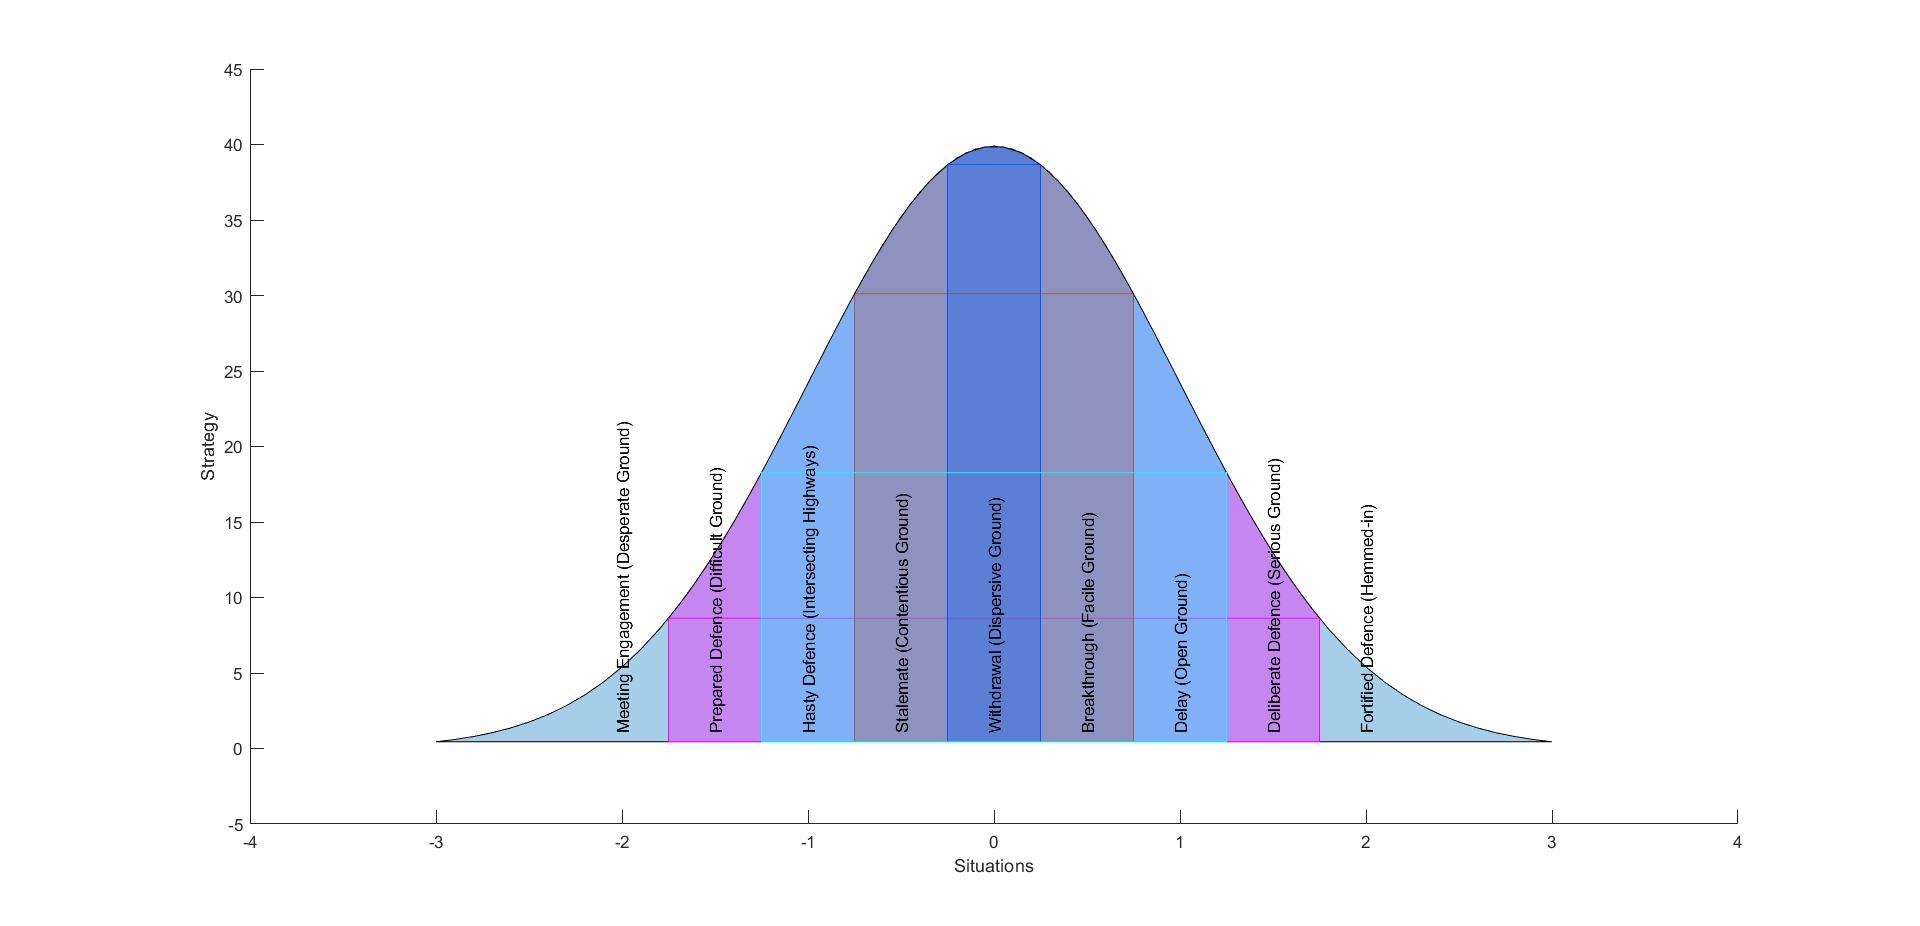
\includegraphics[width=9cm]{situationsvsstrategy.jpg}\\
  \centering
  \caption{Situations and Strategy}
% \end{figure}
\end{sidewaysfigure}

The Matlab Code for generating this figure 
\newpage

 
\tiny
\lstinputlisting[language=Octave]{Untitled.m}
\normalsize
\newpage
\subsection{Theorem-4\\Art of Studying Circumstances }
Consider the battle
\begin{equation}
\begin{split}
    &\Dot{CP_1}=af(CP_1)+bg(CP_2),\\&\Dot{CP_2}=af(CP_2)+bg(CP_1) 
\end{split}
\end{equation}
being $a,b,c,d \in {R}$ and $f$ and $g$ are smooth real function such that $f(0)=g(0)=0$
then:

(i) if $abcd \leq 0$ battle system (23) has no limit cycle.

(ii) Assume that $f$ and $g$ are analytically
\begin{equation}
\begin{split}
  &f(CP_1)=(CP_1)^{{2k}-1}+O(CP_1)^{2l} \text{and} \\&  \Dot{CP_2}=(CP_2)^{{2k}-1}+O(CP_2)^{2l}  
\end{split}
\end{equation}
for some positive integer number $k$ and $l$ where $k \neq l$. Then there exits $abcd$ such that system (23) has at least one limit cycle surrounded the origin which whenever exists is hyperbolic.

(iii) there exists $f$ and $g$ such that for same values of $abcd$ system (23) has more than one limit cycle surrounding the origin. More over same values using $g(CP_2)\equiv CP_2$ that is for system (23).
\newpage
\subsection{Theorem-5\\Art of Studying Mood}
Consider the battle
\begin{equation}
\begin{split}
  &\Dot{CP_1}=Af(CP_1)+Bg(CP_2),\\&\Dot{CP_2}=Cf(CP_2)+Dg(CP_1)  
\end{split}
\end{equation}
being $ABCD$ $\in {R}$ and iid random variables with $N(0,1)$ \index{Gaussian! Distribution Function} and where $f$ and $g$ are smooth real function such that $f(0)=g(0)=0$ then the probability that it does not have periodic orbits is greater than or equal to $\frac{1}{2}$. 
Equivalently, the probability of having some limit cycles is smaller than or equal to $\frac{1}{2}$.
then:

(i) if $abcd \leq 0$ battle system (23) has no limit cycle.

(ii) Assume that $f$ and $g$ are analytically
\begin{equation}
\begin{split}
    &f(CP_1)=(CP_1)^{{2k}-1}+O(CP_1)^{2l} \text{and} \\&  \Dot{CP_2}=(CP_2)^{{2k}-1}+O(CP_2)^{2l} 
\end{split}
\end{equation}
for some positive integer number $k$ and $l$ where $k \neq l$. Then there exits $abcd$ such that system (23) has at least one limit cycle surrounded the origin which whenever exists is hyperbolic.

(iii) there exists $f$ and $g$ such that for same values of $abcd$ system (23) has more than one limit cycle surrounding the origin. More over same values using $g(CP_2)\equiv CP_2$ that is for system (23) .




% A predefined \verb"proof" environment is provided by the \texttt{amsthm} package (which is called by the \texttt{interact} class file), as follows:
 % \begin{proof}
% More recent algorithms for solving the semidefinite programming relaxation are particularly efficient, because they explore the structure of the MAX-CUT problem.
the system does not have periodic orbits
$P(ABCD<0)$ $ABCD$ and $-ABCD$ have same distribution $A$,$-A$, $P(ABCD<0)=P(-ABCD<0)=P(ABCD>0)$
Since $P(ABCD=0)=0 P(ABCD>0)=P(-ABCD<0)$=$\frac{1}{2}$, thus the probability of the system pairing at least one limit cycle is $\leq\frac{1}{2}$
 % \end{proof}
\newpage
\subsection{Theorem-6\\Art of Handling Large Masses}
Consider the random combat system
\begin{equation}
   \Dot{CP_1}=A.f(CP_1)+B.CP_2,
   \nonumber
\end{equation}
\begin{equation}
   \Dot{CP_2}=C.f(CP_1)+D.CP_1.
\end{equation}
where $f(CP_1)=\alpha.{CP_1}^k+\\\sum_{k<r<m}f_i(CP_1)^i+\beta(CP_1)^m$, with $\alpha\beta \neq 0$,  $k\leq 0$  odd integers, $m\geq 1$ and $ABCD$ iid $N(0,1)$ random variables, Assume also that x=0 is the unique real root of  $f(CP_1)\\=0.$Then:  

(i) when $k>1$, the probability of having an odd number of limit cycles is 1/8, and the probability of not having limit cycles or having an even number of there is 7/8.

(ii) when $k=1$ and $\beta>0$, the probability of having an odd number of limit cycles is $P^+(\alpha)\leq1/2$ and the probability of not having limit cycles or the probability of having an even number of them is $1-P^+(\alpha)$. Here $ P^+ :{R} \rightarrow$ $(0,1/2)$ is a decreasing further that satisfies 
$\lim_{\alpha\to\infty }P^+(\alpha)=1/2,P^+(0)=1/8,\lim_{\alpha\to\infty }P^+(\alpha)=0 $
given by:-
\\$P^+(\alpha)=\frac{1}{4pi^2}\iiint_T(\alpha) \exp^{-\frac{(a^2+b^2+c^2+d^2)}{2}} $
where \\$T(\alpha)={(a,b,c,d):ad-bc>0;}$ \\${a(a\alpha+d)\leq s}$
when $k=1$ and $\beta \leq 0$, then some results as in item (ii) hold but changing $P^+$ by $P^-$ where $P^+(\alpha)=P^+(-\alpha)$
In all the cases , each limit cycle is counted with its multiplicity.
\newpage

\section{Discussion}
Figures 2 and 3 show the graphs of Soviet and German Tank losses along with the losses estimated through maximum likelihood approach. In this model a single set of parameters are estimated for representing the entire 14 days of the battle.Figures 4 and 5 show the performance of the same model when entire data set is divided into 5 phases. From these figures, it is apparent that fitting the models with division into 5 phases resulted in a much better fit.Figures 6 and 7 show the further improvement in the data set by dividing it into 14 phases where each day is considered as a mini battle. Further, the total losses are divided into two components: Losses due to tank and Losses due to Artillery. The overall SSR and likelihood values are functions of $p_i$’s and $q_i$’s. Figures 8 and 9 shows the 3D surfaces and contour plots of SSR as a function of $p_1$, $q_1$ and $p_2$, $q_2$ respectively.From these figures, we can see that the minimum SSR zone is represented by contours of $1.5E+5$ and $2.5E+5$. Using a grid search in this zone, the best or optimal fit is obtained at $p_1=.129$, $q_1=.404$, $p_2=.138$, $q_2=.136$ with SSR $1.19E+5$. The $a_1$, $b_1$, $a_2$, $b_2$ values corresponding to the optimal fit are\\ $1.14, 0.70, 0.90, 0.95$ respectively.Figures 10 and 11 shows the surface and contour plots of likelihood as a function of $p_1$, $q_1$ and $p_2$, $q_2$ respectively. From these figures, we can see that the zone of maximum likelihood is represented by contours of $6.0E+3$ and $5.0E+3$ with MLE $5.11E+3$.Using a grid search in this zone, the best or optimal fit is obtained at $p_1=.21$, $q_1=.28$, $p_2=.02$, $q_2=.04$. The $a_1$, $b_1$, $a_2$, $b_2$ values corresponding to the optimal fit are $0.99, 0.88, 0.89, 0.96$ respectively.
Table 2 shows the results of Bracken \autocite{Bracken:1995}, Fricker \autocite{Fricker:1998} , Clemen \autocite{Clemens:1997}  and MLE approaches applied on the tank versus tank and artillery data under heterogeneous situation. This table shows the KS statistic for MLE (with 14 divisions) is 0.08674, which is less than any other estimation methods implying that the method of MLE fits better as compared to the other methods. Also, $R^2$ is a measure of goodness of fit. Larger values of $R^2$ implies a good fit to the data. The $R^2$ value of MLE (with 14 divisions) is1. For comparing the efficiency of the different approaches, the root mean square error (\acrshort{rmse}) criteria is used. The RMSE of MLE with 5 divisions is 88.13 and the RMSE of MLE with 14 divisions is .0005, which is found to be the minimum.The RMSE of\\ Clemen’s Newton-Raphson Iteration model is 116.19, which is found to be the maximum. Therefore, efficiency(E) is measured with respect to the RMSE of the MLE with 14 divisions. Thus, the E for MLE is maximum i.e. equal to 1 and E of Clemen’s model is minimum i.e. equal to $4.30E-06$. If the comparison is made among Bracken's, Fricker's and Clemens approaches, we can say that the Bracken approach is better. However, in all the cases the MLE outperforms other approaches. Based on all the GOF measures, it can be concluded that MLE provides better fits.
	In the present research we just demonstrate that if it is possible for mixing two forces it is also applicable for more than two forces. The number of parameters to be estimated increases fourth folded for mixing one additional force. With the estimated parameters, we computed the casualty due to tank component and casualty due to artillery component (See Table 3).When the 14 days Battle data is considered without any division, $a$ and $b$ parameters are significantly small and $a_1>b_1$ which implies German tanks were more effective than Soviet tanks.Similarly, when we compare $a_2$ against $b_2, b_2>a_2$ which implies Soviet artillery were more effective than German artillery. 
Table 4 shows maximised log-likelihood values with divisions into 14 phases where each day is treated as a mini-battle.Table 3 shows the optimal parameters of heterogeneous Lanchester model with an $R^2$ of 1, RMSE of 0.0005, chi-square of 1.9E-5, SSR of 3.3E-6 and MLE of 13202. The parameters are obtained from maximum likelihood estimation of heterogeneous Lanchester model of tank and Artillery data (table 1) from Kursk Database with each day as single phase. The GRG algorithm is applied for maximizing the likelihood function given in equation (9).Also, the parameter estimates $a_i, b_i, p_i, q_i$ are given corresponding to the maximised log-likelihood values with divisions.From this table we can see that the patterns of the parameters for each day of the battle are same for both the sides. In addition the tank component  parameters are seen to be playing major role in the entire duration of the battle. Out of 14 days, 10 days the tank component parameters came out to be the maximum.That’s why the result justified the Battle of Kursk and was correctly termed as the largest tank battle in the history.
\newpage
\section{Conclusions}
Although mathematical formulations are well established for heterogeneous Lanchester model, very few studies have been done to model actual battle scenario. We have developed heterogeneous Lanchester model for Kursk Battle from World War II using tank and artillery data. All the previous studies on Kursk Battle were done to capture the homogeneous weapon system (Tank against Tank or Artillery against Artillery). The working principles of this model were only applicable for homogeneous situation. So extending those models in heterogeneous situation both theoretically and practically were main focus of this book. We have formulated the likelihood expression under heterogeneous situation and applied to fit model under heterogeneous Lanchester model for Kursk database.We have estimated the MLE of the different parameters that are proved to be statistically more accurate. The unfamiliarity to deal with the heterogeneous situation by the previous approaches motivated us to venture the minute details of the Kursk Battle. The estimates are cross-validated to control the problem of the over fitting. Also, these estimates possess the optimal properties of consistency, sufficiency and efficiency. So compared to the previous work, the present book opens up the opportunity for exploring the complicated structure of Kursk Battle of World War II.Figure: ,Directional Field or D-Field Plot: Considerable insight into the Combat system described through equations as referred in the table 6 can be gained by examining the behaviour of the differential equations through the use of plots known as Directional field plots or D-field plots. The graph gives  an idea whether the system is going to stable at a point or diverges without actually knowing the solutions. These graphs show the convergent and divergent properties of the battles.


% \begin{table}[]

\begin{sidewaystable}
\centering
% \begin{longtable}[c]{| c | c |}
\tiny
\caption{Comparison of different estimation methods}

% \caption{Comparison of different estimation methods with respect to common Goodness-of-fit measures such as sum of square residuals (SSR), Kolmogorov-Smirnov (KS) Statistic, $\chi^2$   and R-square ($R^2$), root mean square error (RMSE) and efficiency($E^2$) from homogeneous tank against tank data of the Kursk battle.}\label{table}
{\begin{tabular}{|p{.1cm}|c|p{.8cm}|c|c|c|}   \hline\hline
\bf{Sl. No.} & \bf{Approaches} &	\bf{SSR/log-Likelihood}	& \bf{KS} & \bf{$\chi^2$} & $\bf{R^2}$  \\
\hline
\hline
1&Bracken\autocite{Bracken:1995}& & & &  \\
\hline
&Model I&1.19E+5&0.1567&2954&\\
\hline
2&Fricker\autocite{Fricker:1998}& & & &  \\
\hline
&Model I&1.29E+5&0.1065&3082&0.44\\
\hline
3&Clemens\autocite{Clemens:1997}& & & &  \\
\hline
&Linear Regression I&1.88E+5&0.1063&3854&0.22\\
\hline
&Newton-Raphson Iteration&1.89E+5&0.1123&3520&0.22\\
\hline
&MLE Log-Likelihood \autocite{Das:2007}& & & &  \\
\hline
4&Without-division&13203&0.1053&2580&0.71\\
\hline
5&With-divisions (4 phases)&13313&0.0909&2670&0.82\\
\hline
\hline
\end{tabular}}
\end{sidewaystable}
% \end{table}

\begin{sidewaystable}
\centering
% \begin{longtable}[c]{| c | c |}
\tiny
\caption{Continue...Comparison of different estimation methods}\label{table}

% \caption{Comparison of different estimation methods with respect to common Goodness-of-fit measures such as sum of square residuals (SSR), Kolmogorov-Smirnov (KS) Statistic, $\chi^2$   and R-square ($R^2$), root mean square error (RMSE) and efficiency($E^2$) from homogeneous tank against tank data of the Kursk battle.}\label{table}
{\begin{tabular}{|p{.1cm}|c|p{.8cm}|c|}   \hline\hline
\bf{Sl. No.} & \bf{Approaches} &		$\bf{RMSE}$ &	${\bf{E^2}}$ \\
\hline
\hline
1&Bracken\autocite{Bracken:1995}& &  \\
\hline
&Model I&92.19&0.9559\\
\hline
2&Fricker\autocite{Fricker:1998}& &  \\
\hline
&Model I&95.99&0.9181\\
\hline
3&Clemens\autocite{Clemens:1997}& &  \\
\hline
&Linear Regression I&115.88&0.7605\\
\hline
&Newton-Raphson Iteration&116.19&0.7584\\
\hline
&MLE Log-Likelihood \autocite{Das:2007}& &  \\
\hline
4&Without-division&89.72&0.9822\\
\hline
5&With-divisions (4 phases)&88.13&1\\
\hline
\hline
\end{tabular}}
\end{sidewaystable}
% \end{table}


\begin{sidewaystable}
\centering
\tiny
%\centering
\caption{Maximization of likelihood estimation with divisions from homogeneous tank against tank data of Kursk battle. }
%\label{tabladeseables}
{\begin{tabular}{|c|c|c|c|c|c|c|}   \hline\hline
\bf{Sl. No.} & \bf{Likelihood} &	\bf{a}	& \bf{b} & \bf{$p$} & \bf{q} \\
\hline
\hline
Phase 1	&2621.35	&0.9031	&1.0887	&0.4793&	0.3079\\
\hline
Phase 2	&6169.72	&1.1327	&0.7884	&0.1418	&0.4720\\
\hline
Phase 3	&2354.21	&1.0300	&0.8816	&0.3889	&0.4838\\
\hline
Phase 4	&2168.54	&1.0221	&0.8939	&0.2793	&0.3483\\
\hline
\end{tabular}}
%\tabnote{\textsuperscript{a}This footnote shows how to include
% footnotes to a table if required.}
% \label{sample-table}
\end{sidewaystable}

\begin{sidewaystable}
\centering
\tiny
%\centering
\caption{The Parameters of Heterogeneous Lanchester Model. The parameters are obtained from maximum likelihood estimation from heterogeneous tank against tank and artillery data of Kursk battle with each day as single phase.}
%\label{tabladeseables}
{\begin{tabular}{|c|c|c|c|c|c|c|c|c|c|}   \hline\hline
phase & Likelihood  &	\bf${a_1}$ &	\bf${a_2}$ &	\bf${b_1}$&	\bf${b_2}$	 \\
\hline
\hline
Phase I &1232.743& 0.929& 0.456& 0.935& 1.395\\
\hline
Phase II &1559.505 &0.795 &0.670 &1.119 &1.188 \\
\hline
Phase III& 1639.509& 1.062 &1.021& 0.808 &0.887\\
\hline
Phase IV &1894.731& 0.989 &1.133 &0.870 &0.753 \\
\hline
Phase V &1895.489 &1.140 &0.882& 0.815 &0.979 \\
\hline
Phase VI &729.8373 &1.301 &0.897 &0.534 &0.967 \\
\hline
Phase VII &725.2296 &1.151 &0.886 &0.724& 0.972 \\
\hline
Phase VIII& 2432.035 &1.290 &1.332 &0.568& 0.516\\
\hline
Phase IX &613.6283 &1.196& 0.889 &0.714 &0.967 \\
\hline
Phase X &575.0583 &1.270& 0.906 &0.612 &0.960 \\
\hline
Phase XI &608.3638 &1.017& 0.904& 0.888& 0.972\\
\hline
Phase XII &111.104 &0.996 &0.891 &0.885 &0.968\\
\hline
Phase XIII &121.6035 &1.369 &0.907& 0.266 &0.936\\
\hline
Phase XIV &297.3759 &1.550 &0.911 &0.119 &0.945 \\
\hline
\hline
\end{tabular}}
% \label{sample-table}
\end{sidewaystable}

\begin{sidewaystable}
\centering
\tiny
%\centering
\caption{Continue...The Parameters of Heterogeneous Lanchester Model. The parameters are obtained from maximum likelihood estimation from heterogeneous tank against tank and artillery data of Kursk battle with each day as single phase.}
%\label{tabladeseables}
{\begin{tabular}{|c|c|c|c|c|c|c|c|c|c|}   \hline\hline
phase & Likelihood  &	\bf${p_1}$&	\bf${p_2}$&	\bf${q_1}$&	\bf${q_2}$	 \\
\hline
\hline
Phase I &1232.743& 0.011& 0.467 &5E-11 &0.273\\
\hline
Phase II &1559.505 &0.539 &0.039 &0.182 &0.000\\
\hline
Phase III& 1639.509& 0.015 &0.371 &0.285 &0.377\\
\hline
Phase IV &1894.731& 0.000 &0.352 &0.113 &0.418\\
\hline
Phase V &1895.489 &0.215 &0.024 &0.574 &0.000\\
\hline
Phase VI &729.8373 &0.000 &0.055 &0.660& 0.043\\
\hline
Phase VII &725.2296 &0.164& 0.011 &0.516& 0.000\\
\hline
Phase VIII& 2432.035 &0.020& 0.388 &0.507& 0.416\\
\hline
Phase IX &613.6283 &0.184& 0.000 &0.498& 0.030\\
\hline
Phase X &575.0583 &0.140 &0.072& 0.535 &0.106\\
\hline
Phase XI &608.3638 &0.300 &0.138 &0.390 &0.176\\
\hline
Phase XII &111.104 &0.210 &0.022 &0.282 &0.048\\
\hline
Phase XIII &121.6035 &0.002 &0.000 &0.492 &0.000\\
\hline
Phase XIV &297.3759 &0.007 &0.005 &0.576 &0.01\\
\hline
\hline
\end{tabular}}
% \label{sample-table}
\end{sidewaystable}





% \setcounter{table}{4}
\begin{sidewaystable}
\centering
\tiny
\caption{Fitted Tank Losses and residual sum of square using Heterogeneous Lanchester model. The tank and arty components of the fitted models are obtained through maximum likelihood estimation method from heterogeneous tank against tank and artillery data of Kursk battle.}
%\label{tabladeseables}
{\begin{tabular}{|c|c|c|c|c|c|c|c|c|c|}   \hline\hline
Days & SLossFit	& STank Comp. &	SArty Comp.	& $SResidual^2$	 \\
\hline
\hline
phase 1&	105.00&	1.01&	103.99&	1.66E-08	\\\hline
phase 2	&117.00	&116.12&	0.88&	1.82E-08	\\\hline
phase 3	&259.00	&10.34&	248.66	&9.09E-08\\\hline
phase 4	&315.00	&2.29&312.71&	1.1E-07\\\hline
phase 5	&289.00	&287.95	&1.04	&1.03E-07\\\hline
phase 6	&157.00	&155.19	&1.81&	5.37E-07\\\hline
phase 7	&135.00	&134.04&	0.96	&8.65E-08	\\\hline
phase 8	&414.00	&47.77&	366.23	&1.4E-07\\\hline
phase 9	&117.00	&115.91&	1.09&	2.76E-08\\\hline
phase 10&	118.00&	114.91&	3.09&	2.68E-08\\\hline
phase 11&	96.00&	88.11	&7.89&	4.33E-08\\\hline
phase 12&	27.00&	25.55&	1.45&	2.02E-08\\\hline
phase 13&	42.00	&41.09	& 0.91&	2.43E-07\\\hline
phase 14&	85.00&	83.94&	1.06	&2.64E-07\\\hline

\hline

\end{tabular}}
\end{sidewaystable}

\begin{sidewaystable}
\centering
\tiny
\caption{Continue Fitted Tank Losses and residual sum of square using Heterogeneous Lanchester model. The tank and arty components of the fitted models are obtained through maximum likelihood estimation method from heterogeneous tank against tank and artillery data of Kursk battle.}
%\label{tabladeseables}
{\begin{tabular}{|c|c|c|c|c|c|c|c|c|c|}   \hline\hline
Days & GLossFit	&GTank Comp.	&GArty Comp.	& $GResidual^2$ \\
\hline
\hline
phase 1&		198.00&	1.02&	196.98&	3.72E-08\\\hline
phase 2	&	248.00&	246.47&	1.53&	1.34E-07\\\hline
phase 3	&	121.00&	5.81	&115.19	&3.33E-08\\\hline
phase 4	&	108.00&	1.79&	106.21&	3.9E-08\\\hline
phase 5	&	139.00&	137.86	&1.14&	7.21E-10\\\hline
phase 6	&	36.00	&34.20&	1.81&	3.48E-07\\\hline
phase 7	&	63.00	&61.96	&1.04&	2.05E-08\\\hline
phase 8	&	98.00	&15.18&	82.82	&4.39E-08\\\hline
phase 9	&	57.00	&55.83&	1.17	&1.32E-08\\\hline
phase 10&	46.00	&43.08&	2.92&	1.06E-08\\\hline
phase 11&	79.00	&72.21	&6.79&	7.96E-10\\\hline
phase 12&	23.00&	21.50&	1.50&	9.59E-09\\\hline
phase 13&	7.00&	6.06	&0.94	&5.48E-09\\\hline
phase 14&	6.00&	4.91&	1.09&	9.07E-07\\\hline

\hline

\end{tabular}}\label{landtab}
\end{sidewaystable}




% \setcounter{table}{6}
\begin{sidewaystable}
\centering
% \begin{table}
\tiny
\caption{Applications of Lanchester's Differential Equations on various Battles}
{\begin{tabular}{|p{0.1cm}|p{1.7cm}|p{5cm}|}\hline\hline
\tiny
\RaggedLeft
%\toprule%
%& \multicolumn{3}{@{}c@{}}{Element 1\footnotemark[1]}& \multicolumn{3}{@{}c@{}}{Element\footnotemark[2]} \\\cmidrule{2-4}\cmidrule{5-7}%
Sl. No. & Battle Name	& Equations   \\
\hline
1& Iwo Jima\autocite{Rbloggers:2016} &$\frac{d(USA)}{dt}=-a_{USA}.(Jap)^p(USA)^q,\frac{d(Jap)}{dt}=-b_{Jap}.(Jap)^q(USA)^p$,\\
\hline
2&Battle of Atlantic\autocite{Washburn:2000} &$\Dot{M}=2(S/E),\Dot{S}=-(1.6\times{10^{-6}}E+8\times10^{-4})S+.7,\Dot{E}=3.2\times{10^{-7}}S{E+.5}$ \\\hline
3&Battle of Trafalgar\autocite{Kingman2002StochasticAO},\autocite{DanTeague},\autocite{1231440} & $\Dot{A}=-bB,\Dot{B}=-aA$  \\\hline
4&Battle of Kursk\autocite{LukasTurkes:2004} &$\Dot{S}=-adS^pG^q,\Dot{G}=-b(\frac{1}{d})S^qG^p$  \\\hline
5&Battle of Ardennes\autocite{Bracken:1995} &$\Dot{S}=-adS^pG^q,\Dot{G}=-b(\frac{1}{d})S^qG^p$  \\\hline
6&Battle of Britain\autocite{JohsonMackey:2011} &$\Dot{B}=-aB^pG^q,\Dot{G}=-bB^qG^p$ \\\hline
% \hline
%\botrule
\end{tabular}}
%\footnotetext{Note: This is an example of table footnote this is an example of table footnote this is an example of table footnote this is an example of~table footnote this is an example of table footnote.}
%\footnotetext[1]{This is an example of table footnote.}
\end{sidewaystable}
% \end{table}

\begin{sidewaystable}
\centering
% \begin{table}
\tiny
\caption{Continue...Applications of Lanchester's Differential Equations on various Battles}

{\begin{tabular}{|p{0.1cm}|p{1.7cm}|p{5cm}|}\hline\hline
\tiny
%\toprule%
%& \multicolumn{3}{@{}c@{}}{Element 1\footnotemark[1]}& \multicolumn{3}{@{}c@{}}{Element\footnotemark[2]} \\\cmidrule{2-4}\cmidrule{5-7}%
\centering
Sl. No. & Battle Name	 & Parameters   \\
\hline
1& Iwo Jima\autocite{Rbloggers:2016}  & $\hat{a_{USA}}=0.0577000,\hat{b_{Jap}}=0.01080927 $\\
\hline
2&Battle of Atlantic\autocite{Washburn:2000}  &$\hat{a}=0.0106,\hat{b}=88787 $ \\\hline
3&Battle of Trafalgar\autocite{Kingman2002StochasticAO},\autocite{DanTeague} &  $A=\sqrt{{A^2}_0-\frac{b}{a}{B^2}_0},B=\sqrt{{B^2}_0-\frac{a}{b}{A^2}_0}$ \\\hline
4&Battle of Kursk\autocite{LukasTurkes:2004} &$\hat{p}=5.87,\hat{q}=1,\hat{a}=4.9\times10^{-35},\hat{b}=3.52\times10^{-36}, \hat{d}=1.02 $ \\\hline
5&Battle of Ardennes\autocite{Bracken:1995} &$\hat{p}=0.91,\hat{q}=-0.61,\hat{a}=4.9\times10^{-35},\hat{b}=3.52\times10^{-36}, \hat{d}=1.02 $ \\\hline
6&Battle of Britain\autocite{JohsonMackey:2011}  &$\hat{a}=-5.4E^{-4},\hat{b}=-(-8.4\times{10^{-4}},\hat{p}=1.2,\hat{q}=0.9$\\\hline
% \hline
%\botrule
\end{tabular}}
%\footnotetext{Note: This is an example of table footnote this is an example of table footnote this is an example of table footnote this is an example of~table footnote this is an example of table footnote.}
%\footnotetext[1]{This is an example of table footnote.}
\end{sidewaystable}




\begin{figure}
\centering
\subfloat[German's Tanks Losses]{%
\resizebox*{3cm}{!}{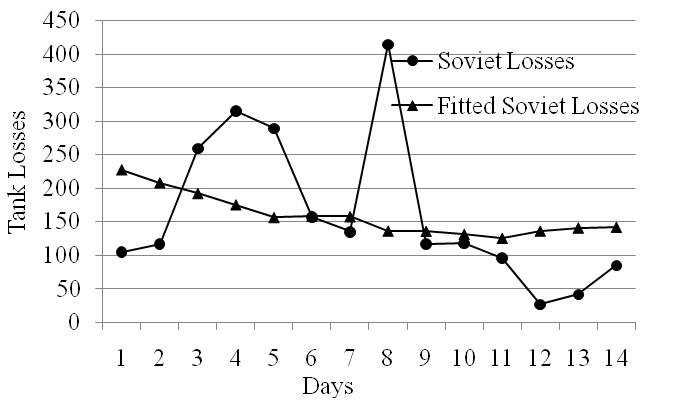
\includegraphics{figure1.png}}}\hspace{1pt}
\subfloat[Soviet's Tanks Losses]{%
\resizebox*{3cm}{!}{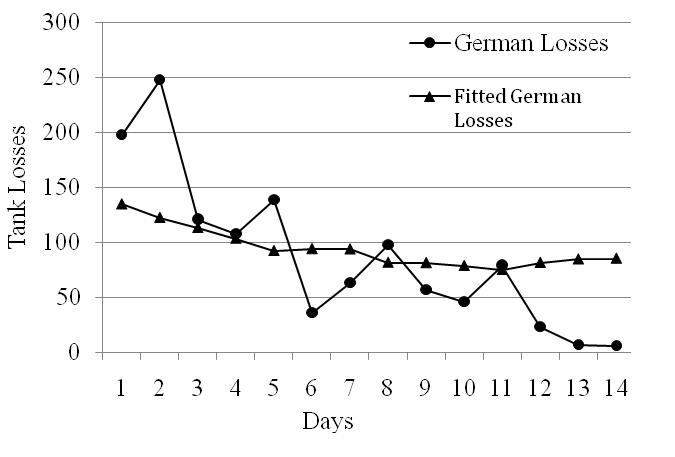
\includegraphics{figure2.png}}}
\caption{Fitted Losses plotted versus real losses for the (a) German's Tanks Losses  (b) Soviet's Tanks Losses without any division of the Battle of Kursk of WW II.} 
\end{figure}

\begin{figure}

\centering
\subfloat[German's Tanks Losses]{%
\resizebox*{3cm}{!}{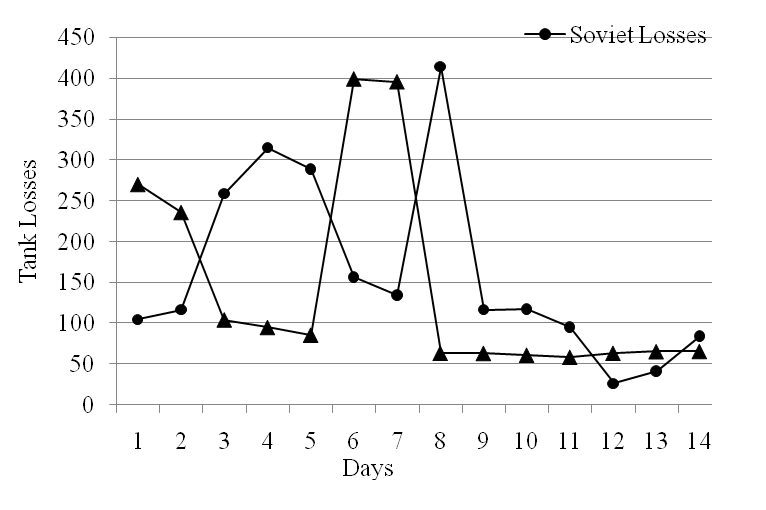
\includegraphics{figure3.png}}}\hspace{5pt}
\subfloat[Soviet's Tanks Losses]{%
\resizebox*{3cm}{!}{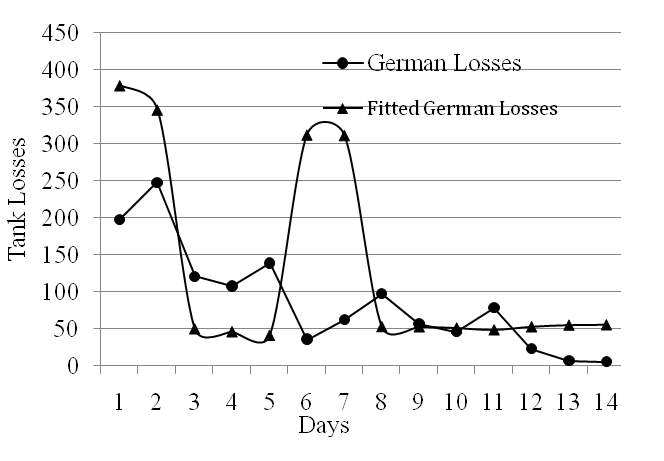
\includegraphics{figure4.png}}}
\caption{
% Fitted tank Losses plotted versus real tank losses for the (a) Soviets and (b) German's with division over multiple phases of the Battle of Kursk of WW II. 
The multiple phases are arranged as divisions 
% 1(with day 1, 2), division 2 (with day 3-7), division 3 (with day 8), division 4 (with day 9-14).
} 
\end{figure}




\begin{figure}
\centering
\subfloat[German's Tanks Losses]{%
\resizebox*{3cm}{!}{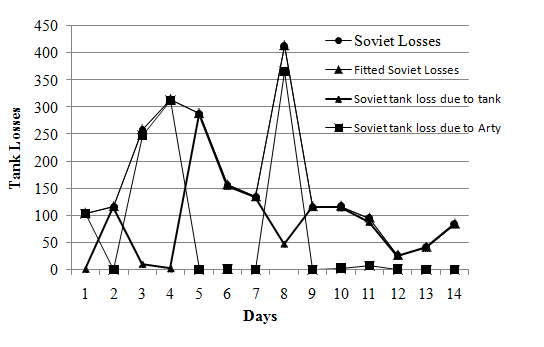
\includegraphics{figure5.png}}}\hspace{5pt}
\subfloat[Soviet's Tanks Losses]{%
\resizebox*{3cm}{!}{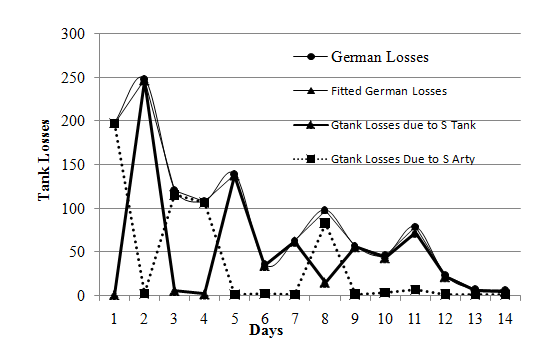
\includegraphics{figure6.png}}}
\caption{
% Fitted (a) Soviet's tank losses due to German's and (b) German's tank losses due to Soviet's tank and artillery using heterogeneous Lanchester model of the Battle of Kursk of WW II.
Total losses are divided into two components, losses due to tank and losses due to arty.} 
\end{figure}


\begin{figure}
\centering
\subfloat[German's Tanks Losses]{%
\resizebox*{3cm}{!}{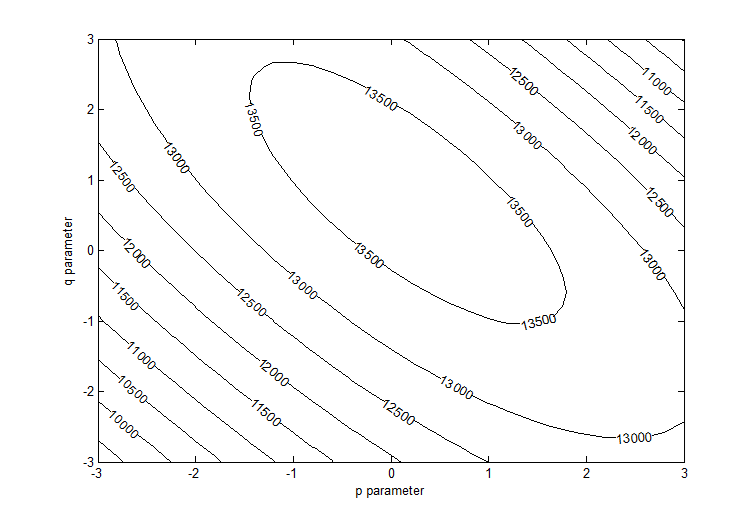
\includegraphics{figure7.png}}}\hspace{5pt}
\subfloat[Soviet's Tanks Losses]{%
\resizebox*{3cm}{!}{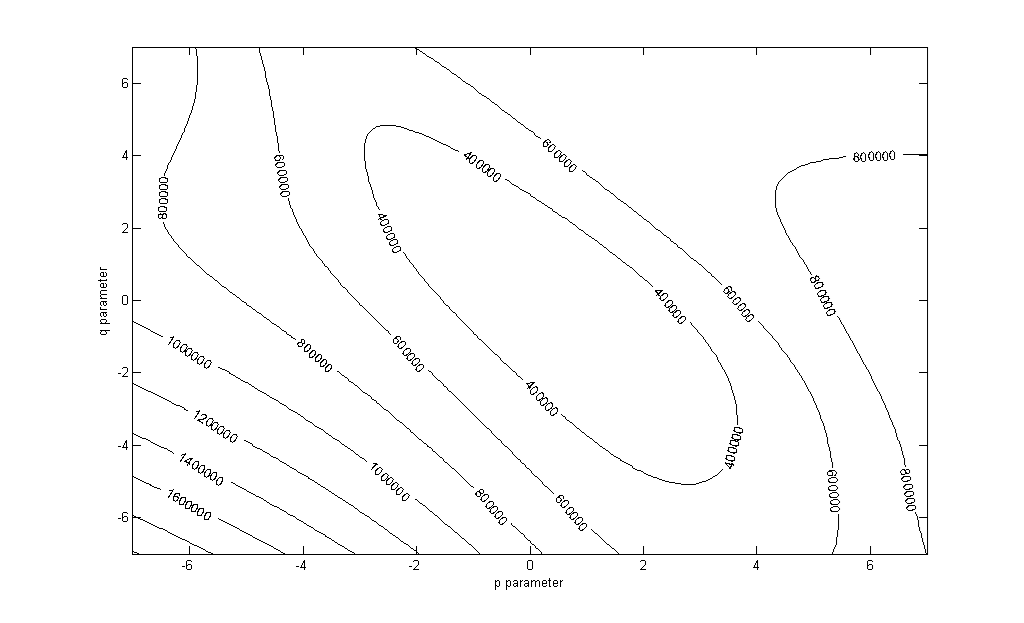
\includegraphics{figure8.png}}}
\caption{Contour plot of (a) Log-likelihood and (b) SSR values for the tank data of Soviet and German sides of the Battle of Kursk of WW II. 
% The p and q values are varied between -3 (-6) and 3 (6) . The parameters are estimated using the MLE and  the Least Square approaches.
} 
\end{figure}

\begin{figure}
\centering
\subfloat[German's Tanks Losses]{%
\resizebox*{4cm}{!}{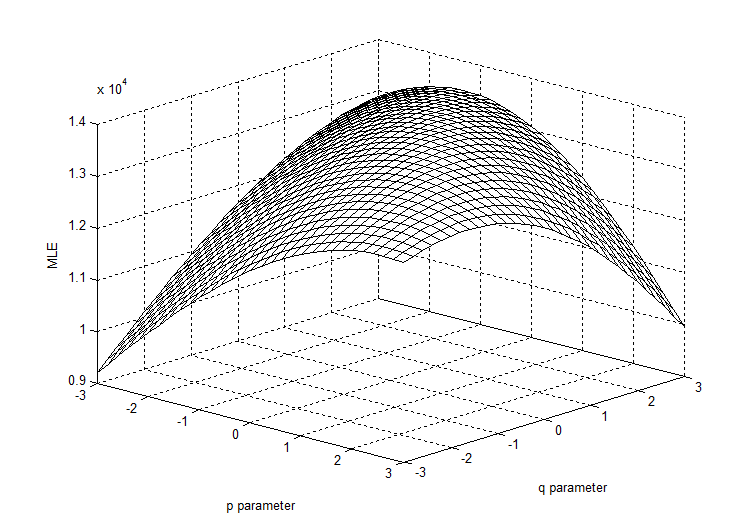
\includegraphics{figure9.png}}}\hspace{5pt}
\subfloat[Soviet's Tanks Losses]{%
\resizebox*{4cm}{!}{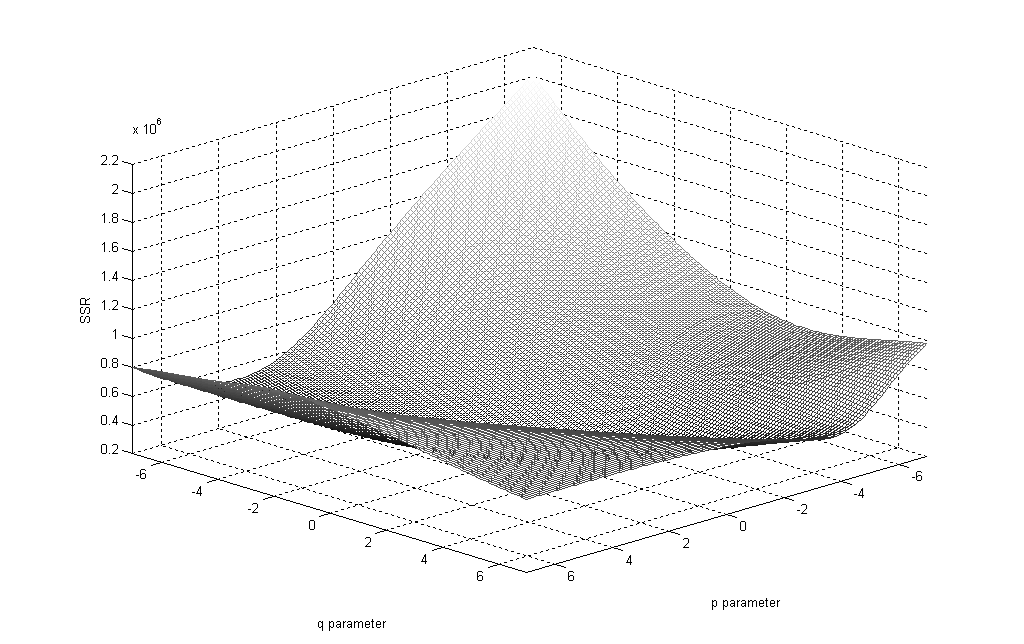
\includegraphics{figure10.png}}}
\caption{
3D plot of (a) Log-likelihood (b) SSR 
% values for the tank data of the Battle of Kursk of WW II.
% , p and q  values are varied between -3(-6) to 3(6), a and b values depend on p and q. The parameters are estimated using the MLE approach.
} 
\end{figure}

\begin{figure}
\centering
\subfloat[Iwo-Jima\autocite{Rbloggers:2016}]{%
\resizebox*{2cm}{!}{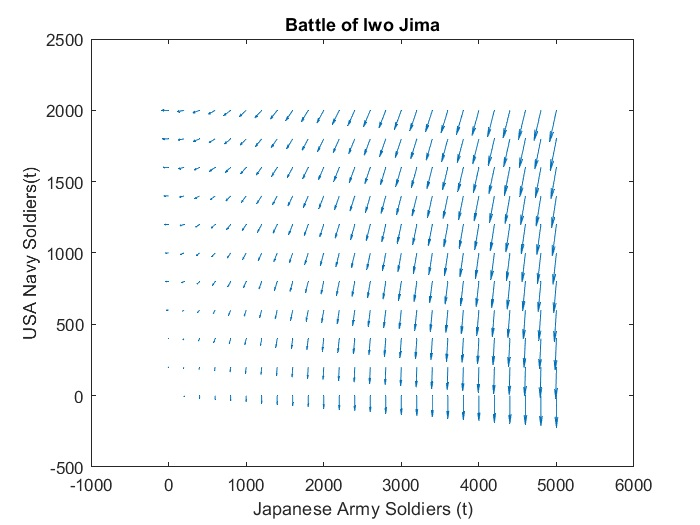
\includegraphics{Iwo-Jima.jpg}}}%\hspace{1pt}
\subfloat[Atlantic \autocite{Washburn:2000}]{%
\resizebox*{2cm}{!}{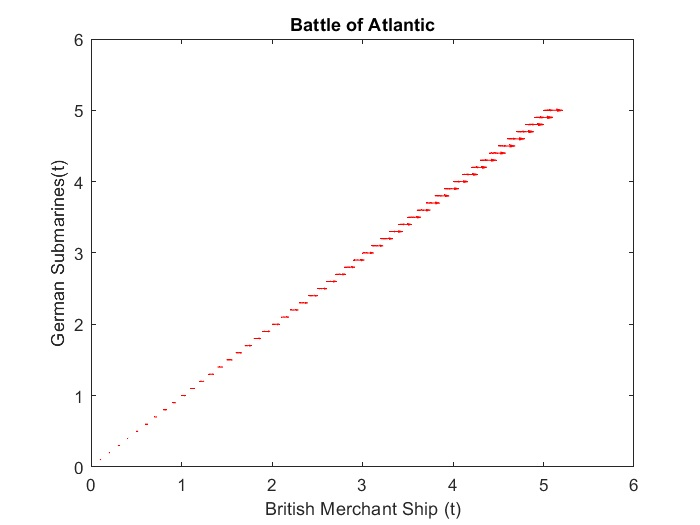
\includegraphics{Atlantic.jpg}}}
\subfloat[Trafalgar \autocite{Kingman2002StochasticAO}]{%
\resizebox*{2cm}{!}{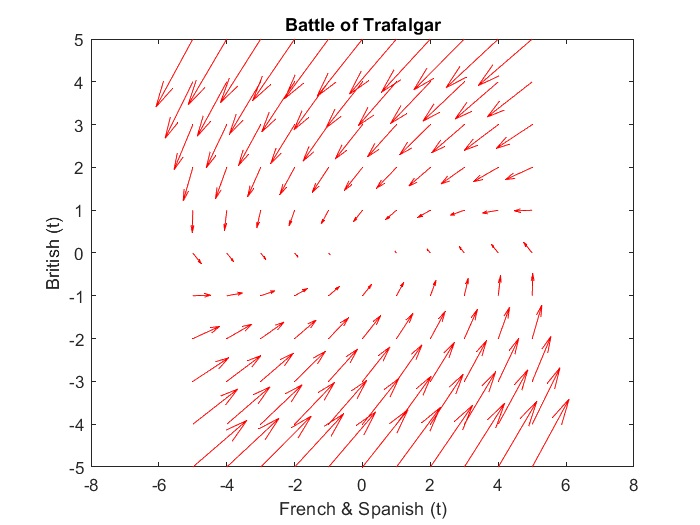
\includegraphics{Trafalgar.jpg}}}\hspace{1pt}
\subfloat[Kursk \autocite{LukasTurkes:2004}]{%
\resizebox*{2cm}{!}{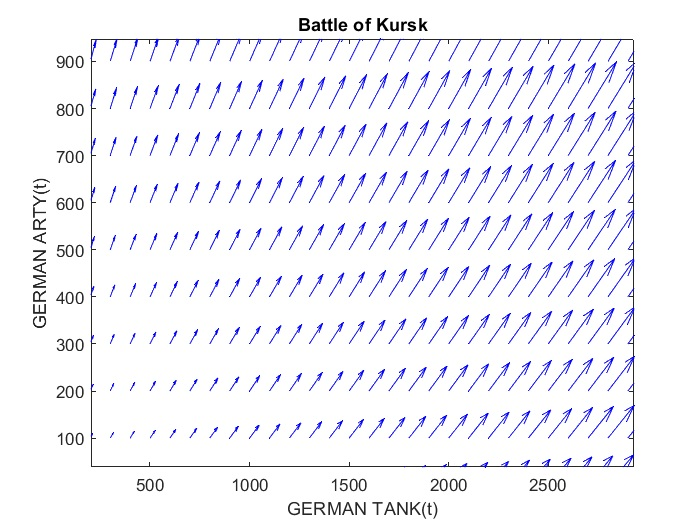
\includegraphics{Kursk.jpg}}}%\hspace{1pt}
\subfloat[Ardennes\autocite{Bracken:1995}]{%
\resizebox*{2cm}{!}{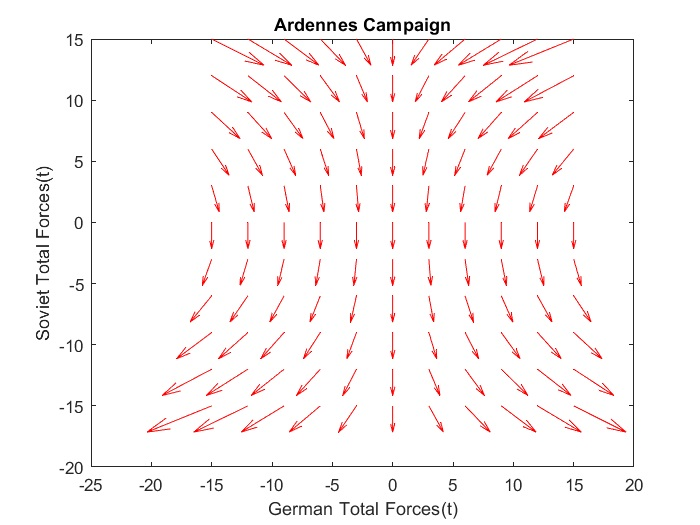
\includegraphics{Ardennes.jpg}}}%\hspace{1pt}
\subfloat[Britain\autocite{JohsonMackey:2011}]{%
\resizebox*{2cm}{!}
{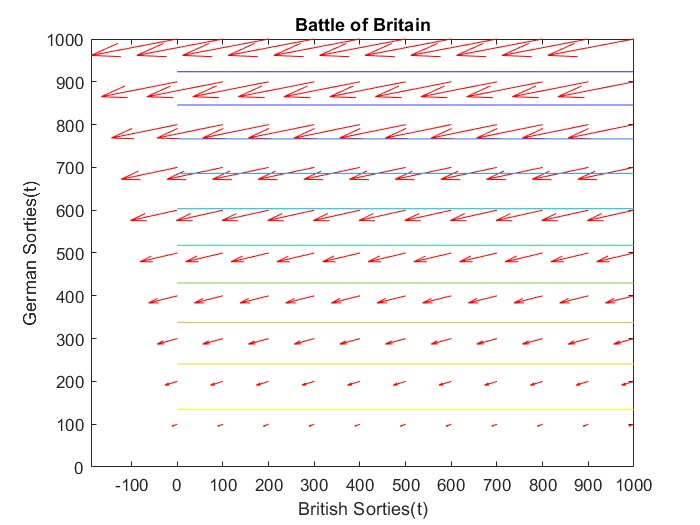
\includegraphics{BB.jpg}}}\hspace{1pt}

\caption{Directional Field or D-Field Plots of different battles
% : Considerable insight into the Combat system described through equations as referred in the table 6 can be gained by examining the behaviour of the differential equations through the use of plots known as Directional field plots or D-field plots. The graph gives  an idea whether the system is going to stable at a point or diverges without actually knowing the solutions. These graphs show the convergent and divergent properties of the battles.
} 
\end{figure}

\begin{figure}
\centering
  % El fichero es un eps y se convierte automaticamente a pdf con eps2pdf package
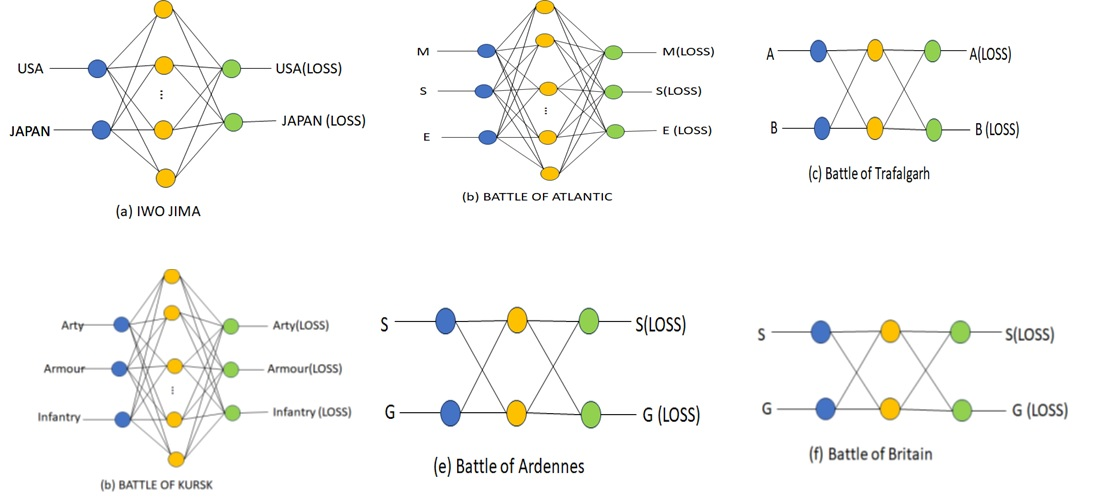
\includegraphics[width=5cm]{DDPGAgent_network.jpg}\\
\caption{Network Structure of different Historical Battles}
\end{figure}
\newpage

\printbibliography
\clearpage
% \printglossary[type=\acronymtype]
\newpage
 % \printglossaries
  \printglossary[title=Glossary And Acronym, toctitle=Glossary And Acronym]
 \footnotesize
\printindex
\newpage
\newpage
\newgeometry{margin=0in,bmargin=0in}
\newgeometry{margin=0in,bmargin=0in}
\voffset=0in
% \vspace*{-0.16in} % only needed for first page
\noindent
\resizebox{\textwidth}{\textheight}
 {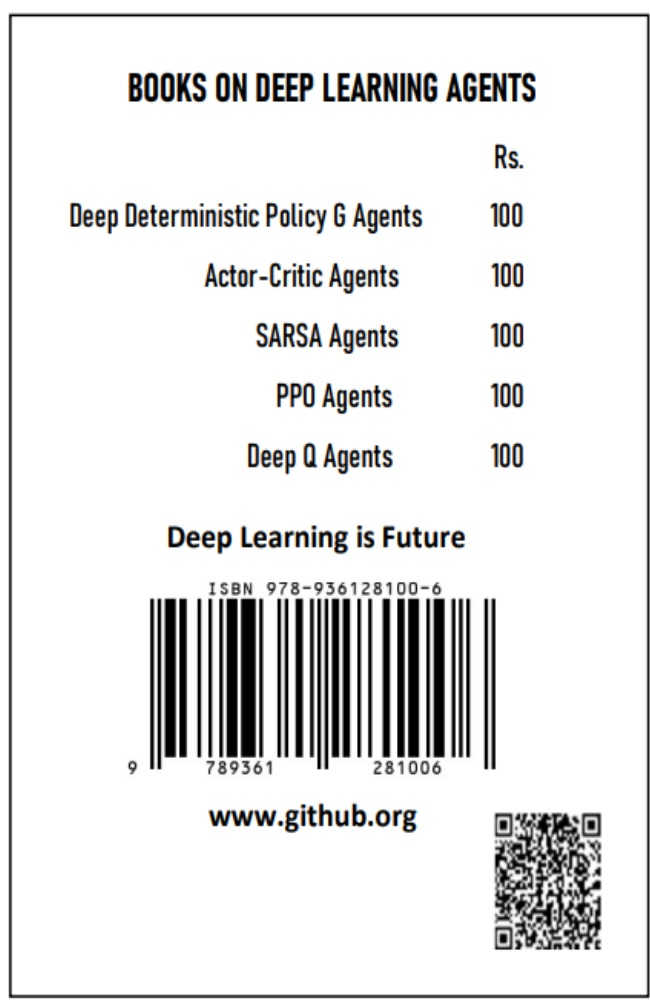
\includegraphics{ddpg_back_cover.jpg}}\hspace*{-\textwidth}
 % \raisebox{3in}[0in][0in]{\color{white}
 % \makebox[\textwidth][c]{\Huge Text over Image}}
\
\thispagestyle{empty}
\addtocounter{page}{-1}%
 \newpage
% \RaggedLeft
 % 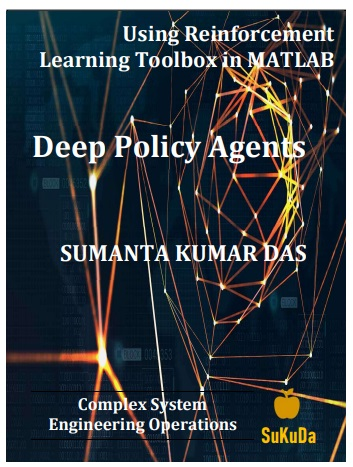
\includegraphics[width=\paperwidth,height=\paperheight]{deep_cover_front.jpg}




\end{document}
% \subsection{References} 
% \label{}



% \medskip
% %\printbibliography
% In order to assist authors in the process of preparing a manuscript for a journal, the Taylor \& Francis `\textsf{Interact}' layout style has been implemented as a \LaTeXe\ class file based on the \texttt{article} document class. A \textsc{Bib}\TeX\ bibliography style file and a sample bibliography are also provided in order to assist with the formatting of your references.

% Commands that differ from or are provided in addition to standard \LaTeXe\ are described in this document, which is \emph{not} a substitute for a \LaTeXe\ tutorial.

% The \texttt{interactnlmsample.tex} file can be used as a template for a manuscript by cutting, pasting, inserting and deleting text as appropriate, using the preamble and the \LaTeX\ environments provided (e.g.\ \verb"\begin{abstract}", \verb"\begin{keywords}").


% \subsection{The \textsf{Interact} class file}\label{class}

% The \texttt{interact} class file preserves the standard \LaTeXe\ interface such that any document that can be produced using \texttt{article.cls} can also be produced with minimal alteration using the \texttt{interact} class file as described in this document.

% If your article is accepted for publication it will be typeset as the journal requires in Minion Pro and/or Myriad Pro. Since most authors will not have these fonts installed, the page make-up is liable to alter slightly with the change of font. Also, the \texttt{interact} class file produces only single-column format, which is preferred for peer review and will be converted to two-column format by the typesetter if necessary during preparation of the proofs. Please therefore do not try to match the typeset format exactly, but use the standard \LaTeX\ fonts instead and ignore details such as slightly long lines of text or figures/tables not appearing in exact synchronization with their citations in the text: these details will be dealt with by the typesetter. Similarly, it is unnecessary to spend time addressing warnings in the log file -- if your .tex file compiles to produce a PDF document that correctly shows how you wish your paper to appear, such warnings will not prevent your source files being imported into the typesetter's program.


% \subsection{Submission of manuscripts prepared using \emph{\LaTeX}}

% Manuscripts for possible publication should be submitted to the Editors for review as directed in the journal's Instructions for Authors, and in accordance with any technical instructions provided in the journal's ScholarOne Manuscripts or Editorial Manager site. Your \LaTeX\ source file(s), the class file and any graphics files will be required in addition to the final PDF version when final, revised versions of accepted manuscripts are submitted.

% Please ensure that any author-defined macros used in your article are gathered together in the preamble of your .tex file, i.e.\ before the \verb"\begin{document}" command. Note that if serious problems are encountered in the coding of a document (missing author-defined macros, for example), the typesetter may resort to rekeying it.


% \section{Using the \texttt{interact} class file}

% For convenience, simply copy the \texttt{interact.cls} file into the same directory as your manuscript files (you do not need to install it in your \TeX\ distribution). In order to use the \texttt{interact} document class, replace the command \verb"\documentclass{article}" at the beginning of your document with the command \verb"\documentclass{interact}".

% The following document-class options should \emph{not} be used with the \texttt{interact} class file:
% \begin{itemize}
%   \item \texttt{10pt}, \texttt{11pt}, \texttt{12pt} -- unavailable;
%   \item \texttt{oneside}, \texttt{twoside} -- not necessary, \texttt{oneside} is the default;
%   \item \texttt{leqno}, \texttt{titlepage} -- should not be used;
%   \item \texttt{twocolumn} -- should not be used (see Subsection~\ref{class});
%   \item \texttt{onecolumn} -- not necessary as it is the default style.
% \end{itemize}
% To prepare a manuscript for a journal that is printed in A4 (two column) format, use the \verb"largeformat" document-class option provided by \texttt{interact.cls}; otherwise the class file produces pages sized for B5 (single column) format by default. The \texttt{geometry} package should not be used to make any further adjustments to the page dimensions.

% %If your manuscript has supplementary content you can also use the \verb"interact" class file to prepare all or part of it using the \verb"suppldata" document-class option, which will suppress the `article history' date. This option \emph{must not} be used on any primary content. Note that authors are solely responsible for the preparation of all supplemental material.


% \section{Additional features of the \texttt{interact} class file}

% \subsection{Title, authors' names and affiliations, abstracts and article types}

% The title should be generated at the beginning of your article using the \verb"\maketitle" command.
% In the final version the author name(s) and affiliation(s) must be followed immediately by \verb"\maketitle" as shown below in order for them to be displayed in your PDF document.
% To prepare an anonymous version for double-blind peer review, you can put the \verb"\maketitle" between the \verb"\title" and the \verb"\author" in order to hide the author name(s) and affiliation(s) temporarily.
% Next you should include the abstract if your article has one, enclosed within an \texttt{abstract} environment.
% The \verb"\articletype" command is also provided as an \emph{optional} element which should \emph{only} be included if your article actually needs it.
% For example, the titles for this document begin as follows:
% \begin{verbatim}
% \articletype{ARTICLE TEMPLATE}

% \title{Taylor \& Francis \LaTeX\ template for authors (\textsf{Interact}
% layout + NLM reference style)}

% \author{
% \name{A.~N. Author\textsuperscript{a}\thanks{CONTACT A.~N. Author.
% Email: latex.helpdesk@tandf.co.uk} and John Smith\textsuperscript{b}}
% \affil{\textsuperscript{a}Taylor \& Francis, 4 Park Square, Milton
% Park, Abingdon, UK; \textsuperscript{b}Institut f\"{u}r Informatik,
% Albert-Ludwigs-Universit\"{a}t, Freiburg, Germany} }

% \maketitle

% \begin{abstract}
% This template is for authors who are preparing a manuscript for a
% Taylor \& Francis journal using the \LaTeX\ document preparation system
% and the \texttt{interact} class file, which is available via selected
% journals' home pages on the Taylor \& Francis website.
% \end{abstract}
% \end{verbatim}

% An additional abstract in another language (preceded by a translation of the article title) may be included within the \verb"abstract" environment if required.

% A graphical abstract may also be included if required. Within the \verb"abstract" environment you can include the code
% \begin{verbatim}
% \\\resizebox{25pc}{!}{\includegraphics{abstract.eps}}
% \end{verbatim}
% where the graphical abstract is to appear, where \verb"abstract.eps" is the name of the file containing the graphic (note that \verb"25pc" is the recommended maximum width, expressed in pica, for the graphical abstract in your manuscript).


% \subsection{Abbreviations}

% A list of abbreviations may be included if required, enclosed within an \texttt{abbreviations} environment, i.e.\ \verb"\begin{abbreviations}"\ldots\verb"\end{abbreviations}", immediately following the \verb"abstract" environment.


% \subsection{Keywords}

% A list of keywords may be included if required, enclosed within a \texttt{keywords} environment, i.e.\ \verb"\begin{keywords}"\ldots\verb"\end{keywords}". Additional keywords in other languages (preceded by a translation of the word `keywords') may also be included within the \verb"keywords" environment if required.


% \subsection{Subject classification codes}

% AMS, JEL or PACS classification codes may be included if required. The \texttt{interact} class file provides an \texttt{amscode} environment, i.e.\ \verb"\begin{amscode}"\ldots\verb"\end{amscode}", a \texttt{jelcode} environment, i.e.\ \verb"\begin{jelcode}"\ldots\verb"\end{jelcode}", and a \texttt{pacscode} environment, i.e.\ \verb"\begin{pacscode}"\ldots\verb"\end{pacscode}" to assist with this.


% \subsection{Additional footnotes to the title or authors' names}

% The \verb"\thanks" command may be used to create additional footnotes to the title or authors' names if required. Footnote symbols for this purpose should be used in the order
% $^\ast$~(coded as \verb"$^\ast$"), $\dagger$~(\verb"$\dagger$"), $\ddagger$~(\verb"$\ddagger$"), $\S$~(\verb"$\S$"), $\P$~(\verb"$\P$"), $\|$~(\verb"$\|$"),
% $\dagger\dagger$~(\verb"$\dagger\dagger$"), $\ddagger\ddagger$~(\verb"$\ddagger\ddagger$"), $\S\S$~(\verb"$\S\S$"), $\P\P$~(\verb"$\P\P$").

% Note that any \verb"footnote"s to the main text will automatically be assigned the superscript symbols 1, 2, 3, etc. by the class file.\footnote{If preferred, the \texttt{endnotes} package may be used to set the notes at the end of your text, before the bibliography. The symbols will be changed to match the style of the journal if necessary by the typesetter.}


% \section{Some guidelines for using the standard features of \LaTeX}

% \subsection{Sections}

% The \textsf{Interact} layout style allows for five levels of section heading, all of which are provided in the \texttt{interact} class file using the standard \LaTeX\ commands \verb"\section", \verb"\subsection", \verb"\subsubsection", \verb"\paragraph" and \verb"\subparagraph". Numbering will be automatically generated for all these headings by default.


% \subsection{Lists}

% Numbered lists are produced using the \texttt{enumerate} environment, which will number each list item with arabic numerals by default. For example,
% \begin{enumerate}
%   \item first item
%   \item second item
%   \item third item
% \end{enumerate}
% was produced by
% \begin{verbatim}
% \begin{enumerate}
%   \item first item
%   \item second item
%   \item third item
% \end{enumerate}
% \end{verbatim}
% Alternative numbering styles can be achieved by inserting an optional argument in square brackets to each \verb"item", e.g.\ \verb"\item[(i)] first item"\, to create a list numbered with roman numerals at level one.

% Bulleted lists are produced using the \texttt{itemize} environment. For example,
% \begin{itemize}
%   \item First bulleted item
%   \item Second bulleted item
%   \item Third bulleted item
% \end{itemize}
% was produced by
% \begin{verbatim}
% \begin{itemize}
%   \item First bulleted item
%   \item Second bulleted item
%   \item Third bulleted item
% \end{itemize}
% \end{verbatim}


% \subsection{Figures}

% The \texttt{interact} class file will deal with positioning your figures in the same way as standard \LaTeX. It should not normally be necessary to use the optional \texttt{[htb]} location specifiers of the \texttt{figure} environment in your manuscript; you may, however, find the \verb"[p]" placement option or the \verb"endfloat" package useful if a journal insists on the need to separate figures from the text.

% Figure captions appear below the figures themselves, therefore the \verb"\caption" command should appear after the body of the figure. For example, Figure~\ref{sample-figure} with caption and sub-captions is produced using the following commands:
% \begin{verbatim}
% \begin{figure}
% \centering
% \subfloat[An example of an individual figure sub-caption.]{%
% \resizebox*{5cm}{!}{\includegraphics{graph1.eps}}}\hspace{5pt}
% \subfloat[A slightly shorter sub-caption.]{%
% \resizebox*{5cm}{!}{\includegraphics{graph2.eps}}}
% \caption{Example of a two-part figure with individual sub-captions
%  showing that captions are flush left and justified if greater
%  than one line of text.} \label{sample-figure}
% \end{figure}
% \end{verbatim}

% \begin{figure}
% \centering
% \subfloat[An example of an individual figure sub-caption.]{%
% \resizebox*{5cm}{!}{\includegraphics{graph1.eps}}}\hspace{5pt}
% \subfloat[A slightly shorter sub-caption.]{%
% \resizebox*{5cm}{!}{\includegraphics{graph2.eps}}}
% \caption{Example of a two-part figure with individual sub-captions
%  showing that captions are flush left and justified if greater
%  than one line of text.} \label{sample-figure}
% \end{figure}

% To ensure that figures are correctly numbered automatically, the \verb"\label" command should be included just after the \verb"\caption" command, or in its argument.

% The \verb"\subfloat" command requires \verb"subfig.sty", which is called in the preamble of the \texttt{interactnlmsample.tex} file (to allow your choice of an alternative package if preferred) and included in the \textsf{Interact} \LaTeX\ bundle for convenience. Please supply any additional figure macros used with your article in the preamble of your .tex file.

% The source files of any figures will be required when the final, revised version of a manuscript is submitted. Authors should ensure that these are suitable (in terms of lettering size, etc.) for the reductions they envisage.

% The \texttt{epstopdf} package can be used to incorporate encapsulated PostScript (.eps) illustrations when using PDF\LaTeX, etc. Please provide the original .eps source files rather than the generated PDF images of those illustrations for production purposes.


% \subsection{Tables}

% The \texttt{interact} class file will deal with positioning your tables in the same way as standard \LaTeX. It should not normally be necessary to use the optional \texttt{[htb]} location specifiers of the \texttt{table} environment in your manuscript; you may, however, find the \verb"[p]" placement option or the \verb"endfloat" package useful if a journal insists on the need to separate tables from the text.

% The \texttt{tabular} environment can be used as shown to create tables with single horizontal rules at the head, foot and elsewhere as appropriate. The captions appear above the tables in the \textsf{Interact} style, therefore the \verb"\tbl" command should be used before the body of the table. For example, Table~\ref{sample-table} is produced using the following commands:
% \begin{table}
% \tbl{Example of a table showing that its caption is as wide as
%  the table itself and justified.}
% {\begin{tabular}{lcccccc} \toprule
%  & \multicolumn{2}{l}{Type} \\ \cmidrule{2-7}
%  Class & One & Two & Three & Four & Five & Six \\ \midrule
%  Alpha\textsuperscript{a} & A1 & A2 & A3 & A4 & A5 & A6 \\
%  Beta & B2 & B2 & B3 & B4 & B5 & B6 \\
%  Gamma & C2 & C2 & C3 & C4 & C5 & C6 \\ \bottomrule
% \end{tabular}}
% \tabnote{\textsuperscript{a}This footnote shows how to include
%  footnotes to a table if required.}
% \label{sample-table}
% \end{table}
% \begin{verbatim}
% \begin{table}
% \tbl{Example of a table showing that its caption is as wide as
%  the table itself and justified.}
% {\begin{tabular}{lcccccc} \toprule
%  & \multicolumn{2}{l}{Type} \\ \cmidrule{2-7}
%  Class & One & Two & Three & Four & Five & Six \\ \midrule
%  Alpha\textsuperscript{a} & A1 & A2 & A3 & A4 & A5 & A6 \\
%  Beta & B2 & B2 & B3 & B4 & B5 & B6 \\
%  Gamma & C2 & C2 & C3 & C4 & C5 & C6 \\ \bottomrule
% \end{tabular}}
% \tabnote{\textsuperscript{a}This footnote shows how to include
%  footnotes to a table if required.}
% \label{sample-table}
% \end{table}
% \end{verbatim}

% To ensure that tables are correctly numbered automatically, the \verb"\label" command should be included just before \verb"\end{table}".

% The \verb"\toprule", \verb"\midrule", \verb"\bottomrule" and \verb"\cmidrule" commands are those used by \verb"booktabs.sty", which is called by the \texttt{interact} class file and included in the \textsf{Interact} \LaTeX\ bundle for convenience. Tables produced using the standard commands of the \texttt{tabular} environment are also compatible with the \texttt{interact} class file.


% \subsection{Landscape pages}

% If a figure or table is too wide to fit the page it will need to be rotated, along with its caption, through 90$^{\circ}$ anticlockwise. Landscape figures and tables can be produced using the \verb"rotating" package, which is called by the \texttt{interact} class file. The following commands (for example) can be used to produce such pages.
% \begin{verbatim}
% \setcounter{figure}{1}
% \begin{sidewaysfigure}
% \centerline{\epsfbox{figname.eps}}
% \caption{Example landscape figure caption.}
% \label{landfig}
% \end{sidewaysfigure}
% \end{verbatim}
% \begin{verbatim}
% \setcounter{table}{1}
% \begin{sidewaystable}
%  \tbl{Example landscape table caption.}
%   {\begin{tabular}{@{}llllcll}
%     .
%     .
%     .
%   \end{tabular}}\label{landtab}
% \end{sidewaystable}
% \end{verbatim}
% Before any such float environment, use the \verb"\setcounter" command as above to fix the numbering of the caption (the value of the counter being the number given to the preceding figure or table). Subsequent captions will then be automatically renumbered accordingly. The \verb"\epsfbox" command requires \verb"epsfig.sty", which is called by the \texttt{interact} class file and is also included in the \textsf{Interact} \LaTeX\ bundle for convenience.

% Note that if the \verb"endfloat" package is used, one or both of the commands
% \begin{verbatim}
% \DeclareDelayedFloatFlavor{sidewaysfigure}{figure}
% \DeclareDelayedFloatFlavor{sidewaystable}{table}
% \end{verbatim}
% will need to be included in the preamble of your .tex file, after the \verb"endfloat" package is loaded, in order to process any landscape figures and/or tables correctly.


 
% \noindent This was produced by simply typing:
% \begin{verbatim}
% \begin{proof}
% More recent algorithms for solving the semidefinite programming
% relaxation are particularly efficient, because they explore the
% structure of the MAX-CUT problem.
% \end{proof}
% \end{verbatim}
% Other theorem-like environments (theorem, definition, remark, etc.) need to be defined as required, e.g.\ using \verb"\newtheorem{theorem}{Theorem}" in the preamble of your .tex file (see the preamble of \verb"interactnlmsample.tex" for more examples). You can define the numbering scheme for these structures however suits your article best. Please note that the format of the text in these environments may be changed if necessary to match the style of individual journals by the typesetter during preparation of the proofs.


% \subsection{Mathematics}

% \subsubsection{Displayed mathematics}

% The \texttt{interact} class file will set displayed mathematical formulas centred on the page without equation numbers if you use the \texttt{displaymath} environment or the equivalent \verb"\[...\]" construction. For example, the equation
% \[
%  \hat{\theta}_{w_i} = \hat{\theta}(s(t,\mathcal{U}_{w_i}))
% \]
% was typeset using the commands
% \begin{verbatim}
% \[
%  \hat{\theta}_{w_i} = \hat{\theta}(s(t,\mathcal{U}_{w_i}))
% \]
% \end{verbatim}

% For those of your equations that you wish to be automatically numbered sequentially throughout the text for future reference, use the \texttt{equation} environment, e.g.
% \begin{equation}
%  \hat{\theta}_{w_i} = \hat{\theta}(s(t,\mathcal{U}_{w_i}))
% \end{equation}
% was typeset using the commands
% \begin{verbatim}
% \begin{equation}
%  \hat{\theta}_{w_i} = \hat{\theta}(s(t,\mathcal{U}_{w_i}))
% \end{equation}
% \end{verbatim}

% Part numbers for sets of equations may be generated using the \texttt{subequations} environment, e.g.
% \begin{subequations} \label{subeqnexample}
% \begin{equation}
%      \varepsilon \rho w_{tt}(s,t) = N[w_{s}(s,t),w_{st}(s,t)]_{s},
%      \label{subeqnparta}
% \end{equation}
% \begin{equation}
%      w_{tt}(1,t)+N[w_{s}(1,t),w_{st}(1,t)] = 0,   \label{subeqnpartb}
% \end{equation}
% \end{subequations}
% which was typeset using the commands
% \begin{verbatim}
% \begin{subequations} \label{subeqnexample}
% \begin{equation}
%      \varepsilon \rho w_{tt}(s,t) = N[w_{s}(s,t),w_{st}(s,t)]_{s},
%      \label{subeqnparta}
% \end{equation}
% \begin{equation}
%      w_{tt}(1,t)+N[w_{s}(1,t),w_{st}(1,t)] = 0,   \label{subeqnpartb}
% \end{equation}
% \end{subequations}
% \end{verbatim}
% This is made possible by the \texttt{amsmath} package, which is called by the class file. If you put a \verb"\label" just after the \verb"\begin{subequations}" command, references can be made to the collection of equations, i.e.\ `(\ref{subeqnexample})' in the example above. Or, as the example also shows, you can label and refer to each equation individually -- i.e.\ `(\ref{subeqnparta})' and `(\ref{subeqnpartb})'.

% Displayed mathematics should be given end-of-line punctuation appropriate to the running text sentence of which it forms a part, if required.

% \subsubsection{Math fonts}

% \paragraph{Superscripts and subscripts}
% Superscripts and subscripts will automatically come out in the correct size in a math environment (i.e.\ enclosed within \verb"\(...\)" or \verb"$...$" commands in running text, or within \verb"\[...\]" or the \texttt{equation} environment for displayed equations). Sub/superscripts that are physical variables should be italic, whereas those that are labels should be roman (e.g.\ $C_p$, $T_\mathrm{eff}$). If the subscripts or superscripts need to be other than italic, they must be coded individually.

% \paragraph{Upright Greek characters and the upright partial derivative sign}
% Upright lowercase Greek characters can be obtained by inserting the letter `u' in the control code for the character, e.g.\ \verb"\umu" and \verb"\upi" produce $\umu$ (used, for example, in the symbol for the unit microns -- $\umu\mathrm{m}$) and $\upi$ (the ratio of the circumference of a circle to its diameter). Similarly, the control code for the upright partial derivative $\upartial$ is \verb"\upartial". Bold lowercase as well as uppercase Greek characters can be obtained by \verb"{\bm \gamma}", for example, which gives ${\bm \gamma}$, and \verb"{\bm \Gamma}", which gives ${\bm \Gamma}$.


% \section*{Acknowledgement(s)}

% An unnumbered section, e.g.\ \verb"\section*{Acknowledgements}", may be used for thanks, etc.\ if required and included \emph{in the non-anonymous version} before any Notes or References.


% \section*{Disclosure statement}

% An unnumbered section, e.g.\ \verb"\section*{Disclosure statement}", may be used to declare any potential conflict of interest and included \emph{in the non-anonymous version} before any Notes or References, after any Acknowledgements and before any Funding information.


% \section*{Funding}

% An unnumbered section, e.g.\ \verb"\section*{Funding}", may be used for grant details, etc.\ if required and included \emph{in the non-anonymous version} before any Notes or References.


% \section*{Notes on contributor(s)}

% An unnumbered section, e.g.\ \verb"\section*{Notes on contributors}", may be included \emph{in the non-anonymous version} if required. A photograph may be added if requested.


% \section*{Nomenclature/Notation}

% An unnumbered section, e.g.\ \verb"\section*{Nomenclature}" (or \verb"\section*{Notation}"), may be included if required, before any Notes or References.


% \section*{Notes}

% An unnumbered `Notes' section may be included before the References (if using the \verb"endnotes" package, use the command \verb"\theendnotes" where the notes are to appear, instead of creating a \verb"\section*").


% \section{References}

% \subsection{References cited in the text}

% References should be cited in accordance with US National Library of Medicine (NLM) style. References are cited in the text by a number in square brackets (e.g. [1], [2,4,10], [11--15], \emph{not} [11]--[15]), in the order in which they first appear. For further details on this reference style, see the Instructions for Authors on the Taylor \& Francis website.

% \autocite{Jen05} \autocite{Das2023}Each bibliographic entry has a key, which is assigned by the author and is used to refer to that entry in the text. In this document, the key \verb"Jen05" in the citation form \verb"\autocite{Jen05}" produces `\autocite{Jen05}', and the keys \verb"{Sch02,Wen95}" in the citation form \verb"\autocite{Sch02,Wen95}" produce `\autocite{Sch02,Wen95}'. The citation for a range of bibliographic entries (e.g.\ `\autocite{Sha78,AG98,Smi75,Men05,DCK03,Hor98,Ant03,Zha05,Rog05,SRW05}') will automatically be produced by  \verb"\autocite{Sha78,AG98,Smi75,Men05,DCK03,Hor98,Ant03,Zha05,Rog05,SRW05}". Optional notes may be included at the beginning and/or end of a citation by the use of square brackets, e.g.\ \verb"\autocite[cf.][]{Gau05}" produces `\autocite[cf.][]{Gau05}', \verb"\autocite[p.356]{BGC04}" produces `\autocite[p.356]{BGC04}', and \verb"\autocite[see][p.73-–77]{PI51}" produces `\autocite[see][p.73--77]{PI51}'.


% \subsection{The list of references}

% References should be listed at the end of the main text in the order in which they are first cited in the text. The following list shows some sample references prepared in the Taylor \& Francis NLM style.

% \begin{thebibliography}{99}

% \bibliographystyle{tfnlm}
% \bibliography{interactnlmsample}


% \bibitem{Jen05}%1
% Jenkins~PF. Making sense of the chest x-ray: a hands-on guide. New York (NY):
%   Oxford University Press; 2005.
% \bibitem{Sch02}%2
% Schott~J, Priest~J. Leading antenatal classes: a practical guide. 2nd ed.
%   Boston (MA): Books for Midwives; 2002.

% \bibitem{Wen95}%3
% Wenger~NK, Sivarajan~Froelicher~E, Smith~LK, et~al. Cardiac rehabilitation.
%   Rockville (MD): Agency for Health Care Policy and Research (US); 1995.

% \bibitem{Sha78}%4
% Shakelford~RT. Surgery of the alimentary tract. Philadelphia (PA): W.B.
%   Saunders; 1978. Chapter 2, Esophagoscopy; p. 29--40.

% \bibitem{AG98}%5
% Ambudkar~SV, Gottesman~MM, editors. {ABC} transporters: biomedical, cellular,
%   and molecular aspects. San Diego (CA): Academic Press; 1998. (Methods in
%   enzymology; vol. 292).

% \bibitem{Smi75}%6
% Smith~CE. The significance of mosquito longevity and blood-feeding behaviour in
%   the dynamics of arbovirus infections. Med Biol. 1975;53:288--294.

% \bibitem{Men05}%7
% Meneton~P, Jeunemaitre~X, de~Wardener~HE, et~al. Links between dietary salt
%   intake, renal salt handling, blood pressure, and cardiovascular diseases.
%   Physiol Rev. 2005 Apr;85:679--715.

% \bibitem{DCK03}%8
% Dostorovsky~JO, Carr~DB, Koltzenburg~M, editors. Proceedings of the 10th World
%   Congress on Pain; 2002 Aug~17--22; San Diego, CA. Seattle: IASP Press; c2003.

% \bibitem{Hor98}%9
% Horrobin~DF, Lampinskas~P. The commercial development of food plants used as
%   medicines. In: Prendergast~HD, Etkin~NL, Harris~DR, et~al., editors. Plants
%   for food and medicine. Proceedings of the Joint Conference of the Society for
%   Economic Botany and the International Society for Ethnopharmacology; 1996
%   Jul~1--6; London. Kew (UK): Royal Botanic Gardens; 1998. p. 75--81.

% \bibitem{Ant03}%10
% Antani~S, Long~LR, Thoma~GR, et~al. Anatomical shape representation in spine
%   x-ray images. Paper presented at: VIIP 2003. Proceedings of the 3rd IASTED
%   International Conference on Visualization, Imaging and Image Processing;
%   2003 Sep~8--10; Benalmadena, Spain.

% \bibitem{Zha05}%11
% Zhao~C. Development of nanoelectrospray and application to protein research and
%   drug discovery [dissertation]. Buffalo (NY): State University of New York at
%   Buffalo; 2005.

% \bibitem{Rog05}%12
% Roguskie~JM. The role of \emph{Pseudomonas aeruginosa} 1244 pilin glycan in
%   virulence [master's thesis]. [Pittsburgh (PA)]: Duquesne University; 2005.

% \bibitem{SRW05}%13
% Savage~E, Ramsay~M, White~J, et~al. Mumps outbreaks across England and Wales
%   in 2004: Observational study. BMJ. 2005;330(7500):1119--1120 [cited 2005
%   May~31]; Available from: http://bmj.bmjjournals.com/cgi/reprint/330/7500/1119.

% \bibitem{Gau05}%14
% Gaul~G. When geography influences treament options. Washington Post (Maryland
%   Ed.). 2005 Jul~24;Sect.~A:12 (col.~1).

% \bibitem{BGC04}%15
% Berrino~F, Gatta~G, Crosignani~P. [Case-control evaluation of screening
%   efficacy]. Epidemiol Prev. 2004 Nov--Dec;28:354--359. Italian.

% \bibitem{PI51}%16
% Piaget~J, Inhelder~B. La gen{\`e}se de l'id{\'e}e de hasard chez l'enfant
%   [The origin of the idea of chance in the child]. Paris: Presses
%   Universitaires de France; 1951.

% \end{thebibliography}
% \bigskip
% \noindent This was produced by typing:
% \begin{verbatim}
% \begin{thebibliography}{99}

% \bibitem{Jen05}%1
% Jenkins~PF. Making sense of the chest x-ray: a hands-on guide. New York
%  (NY): Oxford University Press; 2005.

% \bibitem{Sch02}%2
% Schott~J, Priest~J. Leading antenatal classes: a practical guide. 2nd
%  ed. Boston (MA): Books for Midwives; 2002.

% \bibitem{Wen95}%3
% Wenger~NK, Sivarajan~Froelicher~E, Smith~LK, et~al. Cardiac
%  rehabilitation. Rockville (MD): Agency for Health Care Policy and
%  Research (US); 1995.

% \bibitem{Sha78}%4
% Shakelford~RT. Surgery of the alimentary tract. Philadelphia (PA):
%  W.B. Saunders; 1978. Chapter 2, Esophagoscopy; p. 29--40.

% \bibitem{AG98}%5
% Ambudkar~SV, Gottesman~MM, editors. {ABC} transporters: biomedical,
%  cellular, and molecular aspects. San Diego (CA): Academic Press; 1998.
%  (Methods in enzymology; vol. 292).

% \bibitem{Smi75}%6
% Smith~CE. The significance of mosquito longevity and blood-feeding
%  behaviour in the dynamics of arbovirus infections. Med Biol.
%  1975;53:288--294.

% \bibitem{Men05}%7
% Meneton~P, Jeunemaitre~X, de~Wardener~HE, et~al. Links between dietary
%  salt intake, renal salt handling, blood pressure, and cardiovascular
%  diseases. Physiol Rev. 2005 Apr;85:679--715.

% \bibitem{DCK03}%8
% Dostorovsky~JO, Carr~DB, Koltzenburg~M, editors. Proceedings of the
%  10th World Congress on Pain; 2002 Aug~17--22; San Diego, CA. Seattle:
%  IASP Press; c2003.

% \bibitem{Hor98}%9
% Horrobin~DF, Lampinskas~P. The commercial development of food plants
%  used as medicines. In: Prendergast~HD, Etkin~NL, Harris~DR, et~al.,
%  editors. Plants for food and medicine. Proceedings of the Joint
%  Conference of the Society for Economic Botany and the International
%  Society for Ethnopharmacology; 1996 Jul~1--6; London. Kew (UK): Royal
%  Botanic Gardens; 1998. p. 75--81.

% \bibitem{Ant03}%10
% Antani~S, Long~LR, Thoma~GR, et~al. Anatomical shape representation in
%  spine x-ray images. Paper presented at: VIIP 2003. Proceedings of the
%  3rd IASTED International Conference on Visualization, Imaging and
%  Image Processing; 2003 Sep~8--10; Benalmadena, Spain.

% \bibitem{Zha05}%11
% Zhao~C. Development of nanoelectrospray and application to protein
%  research and drug discovery [dissertation]. Buffalo (NY): State
%  University of New York at Buffalo; 2005.

% \bibitem{Rog05}%12
% Roguskie~JM. The role of \emph{Pseudomonas aeruginosa} 1244 pilin
%  glycan in virulence [master's thesis]. [Pittsburgh (PA)]: Duquesne
%  University; 2005.

% \bibitem{SRW05}%13
% Savage~E, Ramsay~M, White~J, et~al. Mumps outbreaks across England and
%  Wales in 2004: Observational study. BMJ. 2005;330(7500):1119--1120
%  [cited 2005 May 31]; Available from:
%  http://bmj.bmjjournals.com/cgi/reprint/330/7500/1119.

% \bibitem{Gau05}%14
% Gaul~G. When geography influences treament options. Washington Post
%  (Maryland Ed.). 2005 Jul~24;Sect.~A:12 (col.~1).

% \bibitem{BGC04}%15
% Berrino~F, Gatta~G, Crosignani~P. [Case-control evaluation of screening
%  efficacy]. Epidemiol Prev. 2004 Nov--Dec;28:354--359. Italian.

% \bibitem{PI51}%16
% Piaget~J, Inhelder~B. La gen{\`e}se de l'id{\'e}e de hasard chez
%  l'enfant [The origin of the idea of chance in the child]. Paris:
%  Presses Universitaires de France; 1951.

% \end{thebibliography}
% \end{verbatim}
% \bigskip
% \noindent Each entry takes the form:
% \begin{verbatim}
% \bibitem{key}%n Bibliography entry
% \end{verbatim}
% where `\texttt{key}' is the tag that is to be used as an argument for the \verb"\autocite{}" commands in the text of the article and `\texttt{Bibliography entry}' is the material that is to appear in the list of references, suitably formatted. The commands
% \begin{verbatim}
% \usepackage[numbers,sort&compress]{natbib}
% \bibpunct[, ]{[}{]}{,}{n}{,}{,}
% \renewcommand\bibfont{\fontsize{10}{12}\selectfont}
% \makeatletter
% \def\NAT@def@citea{\def\@citea{\NAT@separator}}
% \makeatother
% \end{verbatim}
% need to be included in the preamble of your .tex file in order to generate the citations and bibliography as described above.

% Instead of typing the bibliography by hand, you may prefer to create the list of references using a \textsc{Bib}\TeX\ database. The \texttt{tfnlm.bst} file needs to be in your working folder or an appropriate directory, and the lines
% \begin{verbatim}
% \bibliographystyle{tfnlm}
% \bibliography{interactnlmsample}
% \end{verbatim}
% included where the list of references is to appear, where \texttt{tfnlm.bst} is the name of the \textsc{Bib}\TeX\ bibliography style file for Taylor \& Francis' NLM reference style and \texttt{interactnlmsample.bib} is the bibliographic database included with the \textsf{Interact}-NLM \LaTeX\ bundle (to be replaced with the name of your own .bib file). \LaTeX/\textsc{Bib}\TeX\ will extract from your .bib file only those references that are cited in your .tex file and list them in the References section.

% Please include a copy of your .bib file and/or the final generated .bbl file among your source files if your .tex file does not contain a reference list in a \texttt{thebibliography} environment.


% \section{Appendices}

% Any appendices should be placed after the list of references, beginning with the command \verb"\appendix" followed by the command \verb"\section" for each appendix title, e.g.
% \begin{verbatim}
% \appendix
% \section{This is the title of the first appendix}
% \section{This is the title of the second appendix}
% \end{verbatim}
% produces:\medskip

% \noindent\textbf{Appendix A. This is the title of the first appendix}\medskip

% \noindent\textbf{Appendix B. This is the title of the second appendix}\medskip

% \noindent Subsections, equations, figures, tables, etc.\ within appendices will then be automatically numbered as appropriate. Some theorem-like environments may need to have their counters reset manually (e.g.\ if they are not numbered within sections in the main text). You can achieve this by using \verb"\numberwithin{remark}{section}" (for example) just after the \verb"\appendix" command.

% Note that if the \verb"endfloat" package is used on a document containing any appendices, the \verb"\processdelayedfloats" command must be included immediately before the \verb"\appendix" command in order to ensure that the floats belonging to the main body of the text are numbered as such.

% %\processdelayedfloats %%% See above for an explanation of why this command might be needed here.

% \appendix

% \section{Troubleshooting}

% Authors may occasionally encounter problems with the preparation of a manuscript using \LaTeX. The appropriate action to take will depend on the nature of the problem:
% \begin{enumerate}
% \item[(i)] If the problem is with \LaTeX\ itself, rather than with the actual macros, please consult an appropriate \LaTeXe\ manual for initial advice. If the solution cannot be found, or if you suspect that the problem does lie with the macros, then please contact Taylor \& Francis for assistance (\texttt{latex.helpdesk@tandf.co.uk}), clearly stating the title of the journal to which you are submitting.
% \item[(ii)] Problems with page make-up (e.g.\ occasional overlong lines of text; figures or tables appearing out of order): please do not try to fix these using `hard' page make-up commands -- the typesetter will deal with such problems. (You may, if you wish, draw attention to particular problems when submitting the final version of your manuscript.)
% \item[(iii)] If a required font is not available on your system, allow \TeX\ to substitute the font and specify which font is required in a covering letter accompanying your files.
% \end{enumerate}


% \section{Obtaining the template and class file}

% \subsection{Via the Taylor \& Francis website}

% This article template and the \texttt{interact} class file may be obtained via the `Instructions for Authors' pages of selected Taylor \& Francis journals.

% Please note that the class file calls up the open-source \LaTeX\ packages booktabs.sty, epsfig.sty and rotating.sty, which will, for convenience, unpack with the downloaded template and class file. The template calls for natbib.sty and subfig.sty, which are also supplied for convenience.


% \subsection{Via e-mail}

% This article template, the \texttt{interact} class file and the associated open-source \LaTeX\ packages are also available via e-mail. Requests should be addressed to \texttt{latex.helpdesk@tandf.co.uk}, clearly stating for which journal you require the template and class file.
% \begin{figure}
%     \centering
%     \includegraphics[width=13cm]{om.jpg}
%     \caption{Caption}
%     \label{fig:enter-label}
% \end{figure}


